%%%%%%%%%%%%%%%%%%%%%%%%%%%%%%%%%%%%%%%%%%%%%%%%%%%%%%%%%%%%%%%%%%%%%%%%%%%%%%%
% intro.tex: Introduction to the thesis
%%%%%%%%%%%%%%%%%%%%%%%%%%%%%%%%%%%%%%%%%%%%%%%%%%%%%%%%%%%%%%%%%%%%%%%%%%%%%%%%
\chapter{Multicomponent Effects on the Supercritical \ce{CO2} Systems}

\section{Introduction}


\section{Semi-closed \ce{sCO2} cycles} \label{app:sCO2cycle}
    %\section{\ce{sCO2} gas turbine cycle with oxy-combustion} \label{app:sCO2cycle}
    A cycle schematic of semi-closed \ce{sCO2} gas turbine systems is shown in Fig.~\ref{fig1}, which includes the following steps: The mixture of \ce{CO2}/\ce{H2O} with low temperature and low pressure (LTLP) is firstly compressed to a high temperature and high pressure (HTHP) state through the compressor. A cooler is used to remove a majority of the \ce{H2O} at high pressures. %in order to hold on the high turbine inlet temperature. 
    A remover is applied after the cooler to remove the excess \ce{CO2} to conserve the mass in the cycle. The removed \ce{CO2} can be diverted into a bypass stream to serve as a cooling flow around the head and walls of the oxy-combustor (i.e., the ``reactor'' in Fig.~\ref{fig1}). Due to the loss of mass in the remover, the system pressure is reduced. A pump is used as compensation to increase the system pressure to a higher value. As the working fluid with moderate temperature and high pressure (MTHP) goes through a recuperator (i.e., a heat exchanger), the working fluid is heated to a high temperature by the exhaust gas mixture from the turbine. The working fluid enters the reactor (i.e., the oxy-combustor) and mixes with injected \ce{CH4} and \ce{O2}. Then the auto-ignition occurs at around 900 K with high \ce{CO2} concentrations. Herein, it must be noted that the so-called ``supercritical'' is defined based on the \ce{CO2} critical point ($P_c=$73.8 bar, $T_c=$304.2 K) rather than the real mixture critical point.
    \begin{figure}[htbp]
        \begin{center}
            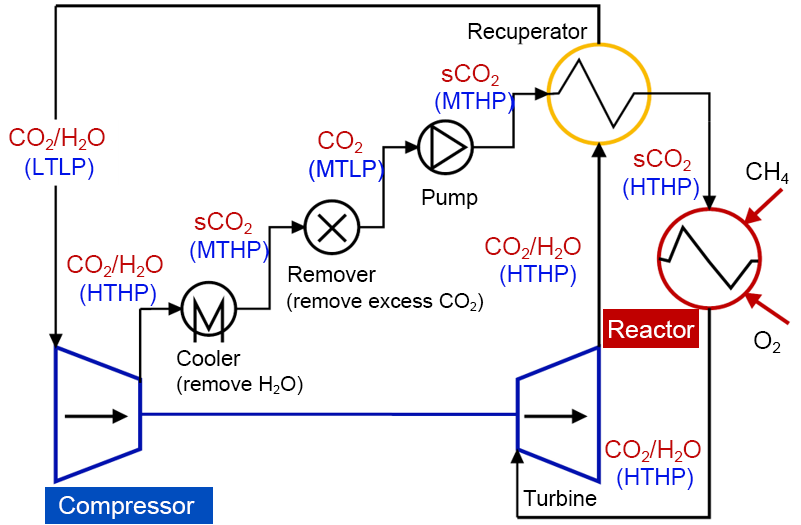
\includegraphics[width=0.6\linewidth]{schematic_cycle.png}
        \end{center}
        \caption{Schematic of a \ce{sCO2} gas turbine cycle with oxy-combustion thermal input.}
        \label{fig1}
    \end{figure}


Semi-closed supercritical carbon dioxide (\ce{sCO2}) oxy-combustion is a promising candidate for the next generation power cycles, since it is one of the potential solutions to effectively remove \ce{CO2} and \ce{NO_x} emissions from power generation. 
In a semi-closed \ce{sCO2} cycle (see details in Appendix~\ref{app:sCO2cycle}), the heat input typically comes from oxy-fuel combustion using either natural gas or syngas from a coal gasification process \citep{mcclung2015comparison}. This direct heating semi-closed \ce{sCO2} power cycle can allow higher turbine inlet temperature than the indirect heating closed \ce{sCO2} cycles to achieve higher efficiency.
The \ce{NO_x} emission is directly avoided by oxy-combustion (i.e., using pure oxygen rather than air as the oxidizer). The combustion products (primarily \ce{CO2} and \ce{H2O}) can be recycled. 
In addition, since the high pressure \ce{sCO2} holds high energy density, it can reduce the equipment size and improve the power density relative to air or oxygen \citep{dostal2004supercritical,ahn2015review}. Although the advantages of the semi-closed \ce{sCO2} gas turbine cycles are evident, the design of these cycles with oxy-combustion thermal input requires extensive knowledge of the real-fluid thermodynamics of multicomponent mixtures at a broad range of temperature and pressure conditions.

In the semi-closed \ce{sCO2} cycles, impurities in \ce{CO2} due to the combustion make it different from the traditional closed \ce{sCO2} cycles, and the semi-closed \ce{sCO2} cycles are no more single-component systems \cite{abdul2017cfd,barak2020ignition}. The impurities, especially components with high critical pressure such as \ce{H2O}, could significantly change the mixture critical point and phase boundary, and consequently, affect the thermodynamic proprieties of the working fluid. Hence, the thermodynamic characteristics of the mixture may deviate a lot from a single component. These effects may trigger phase separation, which may affect the system performance (e.g., thermal efficiency) and/or may cause safety issues. Thus, multicomponent effects on the \ce{sCO2} systems (in terms of the effects of mixture critical point and phase separation) are important and need to be investigated. Supercritical fluid, such as \ce{sCO2}, holds high energy density $\rho e$ near its mixture critical point due to the large variation of density $\rho$, which results in a large change in specific heat capacity $c_p$ for a small temperature change. Therefore, it is better to keep the fluid temperature and pressure close to the mixture critical point to take this special advantage of high energy density to compact the turbomachinery. Accordingly, when designing and analyzing a semi-closed \ce{sCO2} system, an accurate determination of the mixture critical point of a multicomponent mixture becomes very important.

\textbf{Effects of phase separation:}
In the compressor of a semi-closed \ce{sCO2} cycle, phase boundary change caused by multicomponent effects is a potential cause of phase separation. It may lead to compressor blade erosion, which has been widely investigated in traditional steam turbines \cite{ahmad2009experimental} but not in \ce{sCO2} gas turbines. % (see more details in \ref{app:sCO2cycle:compressor}). 
In the \ce{sCO2} oxy-combustor (i.e., the reactor in Fig.~\ref{fig1} of Appendix~\ref{app:sCO2cycle}), phase separation caused by multicomponent effects may also occur due to the mixing between the working fluid (\ce{CO2}/\ce{H2O}) and injected \ce{O2} and \ce{CH4}. For the pure gas phase, the mass mixing time scale is very small due to the large mass diffusivity, and the corresponding ``effective'' ignition delay is also short. For a two-phase state, due to the presence of the liquid phase, the mass diffusivity is decreased, which increases the mass mixing time, but the thermal diffusivity is increased, which reduces the thermal conduction time. In these ways, multicomponent effects may affect the cold ignition in terms of ``effective'' ignition delay. In addition, phase separation may lead to combustion-induced Rapid Phase Transition (cRPT) \citep{basco2013effect}, which causes anomalous high or oscillating pressures to damage the equipment and cause safety issues.

As mentioned above, multicomponent effects are important to understand the semi-closed \ce{sCO2} gas turbine performance, such as thermal efficiency, compressor blade erosion, and ``effective'' ignition delays. However, very few researchers have investigated the influence of impurities (e.g., \ce{H2O}, \ce{CH4}, and \ce{O2}) on the \ce{sCO2} systems \cite{vesely2019effect,pint2018effect}. 
To fill this scientific knowledge gap, the current fundamental study will focus on the multicomponent effects caused by impurities on the \ce{sCO2} systems. % on these effects and raise potential problems.
But please note that the simulation and optimization of the real \ce{sCO2} gas turbine systems (i.e., applied research) is out of the scope of this fundamental research and hence will not be covered in this paper. 

Around the year of 2000, many important works have been done to simulation high-pressure supercritical fluids \cite{oefelein2005thermophysical,bellan2000supercritical,yang2000modeling}. These works majorly used ``dense fluid'' methods to describe the thermodynamic properties in the supercritical region. However, it cannot capture the phase change and multiphase effects (e.g., two-phase thermodynamic and transport properties) near the critical point.
In order to investigate the multiphase thermodynamics of the \ce{sCO2} systems, a vapor-liquid equilibrium (VLE) model \cite{michelsen1982isothermal,michelsen1987multiphase} is used in this study. The VLE model is based on the fundamental thermodynamics theory: Gibbs free energy is at a minimum at equilibrium. Hence, compared to low-pressure vaporization model, the VLE model is more suitable to capture phase boundary near the critical point. In this work, two VLE solvers (i.e., the isothermal-isobaric (TPn) flash solver \cite{michelsen1982isothermal} and isobaric-isenthalpic (HPn) flash solver \cite{michelsen1987multiphase}) are implemented, validated, and verified to predict the phase boundary and real mixture critical point, and simultaneously model the subcritical regime (with the consideration of phase change), the supercritical regime, as well as the transition between them. Thermodynamic and transport properties are evaluated based on the VLE solution, and thermodynamic relation are used to derive the formulas.

VLE model have been used for thermal analysis of various mixture systems. Xu et al. investigated high-pressure VLE at 293 K for \ce{N2}/\ce{CH4}/\ce{CO2} systems \cite{xu1992high}. Perakis et al. modeled the VLE of the \ce{H2O}/ethanol/\ce{CO2} system \cite{perakis2006thermodynamic}. Pappa et al. modeled the VLE of the \ce{CO2}/\ce{H2O} system \cite{pappa2009thermodynamic}. Silvia et al. analyzed the \ce{CO2}-based mixture, and improved accuracy by using an advanced mixing rule \cite{lasala2016vle}. Legoix et al. investigated the mixtures of \ce{CH4}/\ce{CO2} and \ce{CH4}/\ce{CO2}/\ce{H2O} \cite{legoix2017phase}. Although some \ce{CO2}-containing mixtures have been studied using VLE theory, before the present work, detailed VLE thermodynamics analysis of semi-closed \ce{sCO2} systems has never been conducted in the literature, but such analysis is needed to better understand the \ce{sCO2} system performance (e.g., thermal efficiency) and predict potential phase change which may affect ignition or cause safety issues.

Although the VLE theory has been proposed for a long while \cite{hanks1971calculation} and 0D VLE calculation can be done by publicly available software such as the National Institute of Standards and Technology (NIST) REFPROP code \cite{lemmon2018nist}, the development of VLE-based computational fluid dynamics (CFD) solvers to capture high-pressure phase change interacting with flow field just started during the past decade. Matheis and Hickel \cite{matheis2018multi} integrated VLE models to a 3D compressible solver to reveal special breakup behaviors at supercritical conditions, which was also reported in Roy and Segal's experimental results \citep{roy2010experimental} and Ana et al.'s simulation work \citep{star2006numerical}. Yao et al. used the tangent plane distance (TPD) method, a phase stability test method in VLE theory, to investigate the effect of mass diffusion model on phase stability \citep{yao2019molecular}. Ray et al. used the 2D compressible governing equation in the spherical coordinate system to describe droplet fluid dynamics, and integrated a VLE model to investigate the droplet evaporation at high pressures \cite{ray2019two}. Yi et al. developed a compressible four-equation model for multicomponent two-phase flow coupled with VLE solvers. Ma et al. integrated their non-conservative double-flux model \cite{ma2017entropy} to a CFD solver, developed an adaptive scheme by coupling existing quasi-conservative and fully-conservative scheme, and analyzed the mixing behavior of fully conservative and quasi-conservative schemes \citep{ma2019numerical}. Tudisco and Menon developed the formula to handle VLE in multi-component mixtures (i.e., more than two components), and combined the non-conservative double-flux model \cite{ma2017entropy} to a CFD solver to investigate the VLE effects on mixing flows \cite{tudisco2020numerical}. In addition, Tudisco and Menon \cite{tudisco2020vapor} also developed a p$\rho$n VLE solver, and investigated the coupling between thermodynamic and transport properties and governing equations. Different from all the works above, this research integrated VLE solver with a CFD solver based on the PIMPLE algorithm \cite{holzmann2016mathematics}, which is a pressure-based scheme and suitable for ``low-Mach'' CFD simulation (but can also handle up to Mach 2 flows in its new transonic version). This work also developed a novel VLE-based tabulation method to make the VLE-based CFD solver computationally more affordable. 

This work develops a VLE-based CFD simulation framework by coupling a pressure-based CFD solver with the HPn flash solver to capture the phase separation in high-pressure multiphase flows. The thermodynamics analyses (of multicomponent mixtures) and CFD simulations (of a laminar premixed shock tube and turbulent jet-in-crossflows) are then conducted to reveal several mechanisms of phase separation in the \ce{sCO2} systems.

The objectives of this research are:

\noindent$\bullet$ Understanding and quantifying the effects of combustion-relevant impurities (e.g., \ce{H2O}, \ce{CH4}, and \ce{O2}) on the mixture critical points and phase separation in the \ce{sCO2} systems.

\noindent$\bullet$ Understanding and quantifying the effects of phase separation on different thermodynamic properties in the \ce{sCO2} systems.

\noindent$\bullet$ Understanding the mechanisms of phase separation in premixed \ce{sCO2} systems, particularly whether compression or expansion waves can trigger phase separation.

\noindent$\bullet$ Understanding the mechanisms of phase separation in non-premixed \ce{sCO2} systems, particularly whether flow field and mixing processes can trigger phase separation.








\section{Results and Discussion}

To investigate the effects of phase separation in \ce{sCO2} systems, 0D thermodynamics analyses are first performed to discover the conditions under which phase separation could occur (in Sec.~\ref{sec:results:ThermAnalysis}). In Sec.~\ref{sec:results:ShockTube}, 1D shock tube simulations are conducted to understand the effect of the phase change model compared with two models without phase change, and understand the interaction between phase separation and compression/expansion waves. In Sec.~\ref{sec:results:JICF}, we performed 3D jet-in-crossflow LES to discuss the influence of mixing on phase separation. 

\subsection{0D thermodynamics analyses of the \ce{sCO2} systems}
\label{sec:results:ThermAnalysis}

In a real flow, many factors (e.g., boundary condition, turbulence, temperature perturbation) affect the fluid flow, making it difficult to analyze thermodynamic properties. Hence, in this section, 0D thermodynamics analyses are performed to give insights into the thermodynamic properties without the influence of other factors. First, the mixture critical points are calculated to show the influence of impurities in Sec.~\ref{sec:results:combustor:H2O}. Then, the influence of the critical point on thermodynamic properties is discussed in Sec.~\ref{sec:results:combustor:phase}. Since isenthalpic mixing is similar to what often happens in the real \ce{sCO2} systems, in the end, the two-phase region in the isenthalpic mixing process is discussed (in Sec.~\ref{sec:results:combustor:HPn}). 

%\subsubsection{Influence of \ce{H2O} addition on the mixture phase diagrams near the fuel injector}
\subsubsection{Influence of impurities on premixed \ce{sCO2} systems: elevated critical point and retrograde condensation}
\label{sec:results:combustor:H2O}


As discussed before, the injection of fuel (e.g., \ce{CH4}) and oxidizer (e.g., pure \ce{O2} or air) and the combustion products (e.g., \ce{H2O}) can introduce many impurities to the \ce{sCO2} systems. Accordingly, this section will investigate the mixture phase diagrams of \ce{sCO2} systems with different combinations of impurities, including both two-component and three-component systems (also see Appendix~\ref{app:trad} and Sec.~\ref{sec:results:combustor:phase} for four-component systems).

    \begin{figure}[htb]
        \centering
        \subfigure{
            %\begin{minipage}[t]{0.5\linewidth}
            \centering
            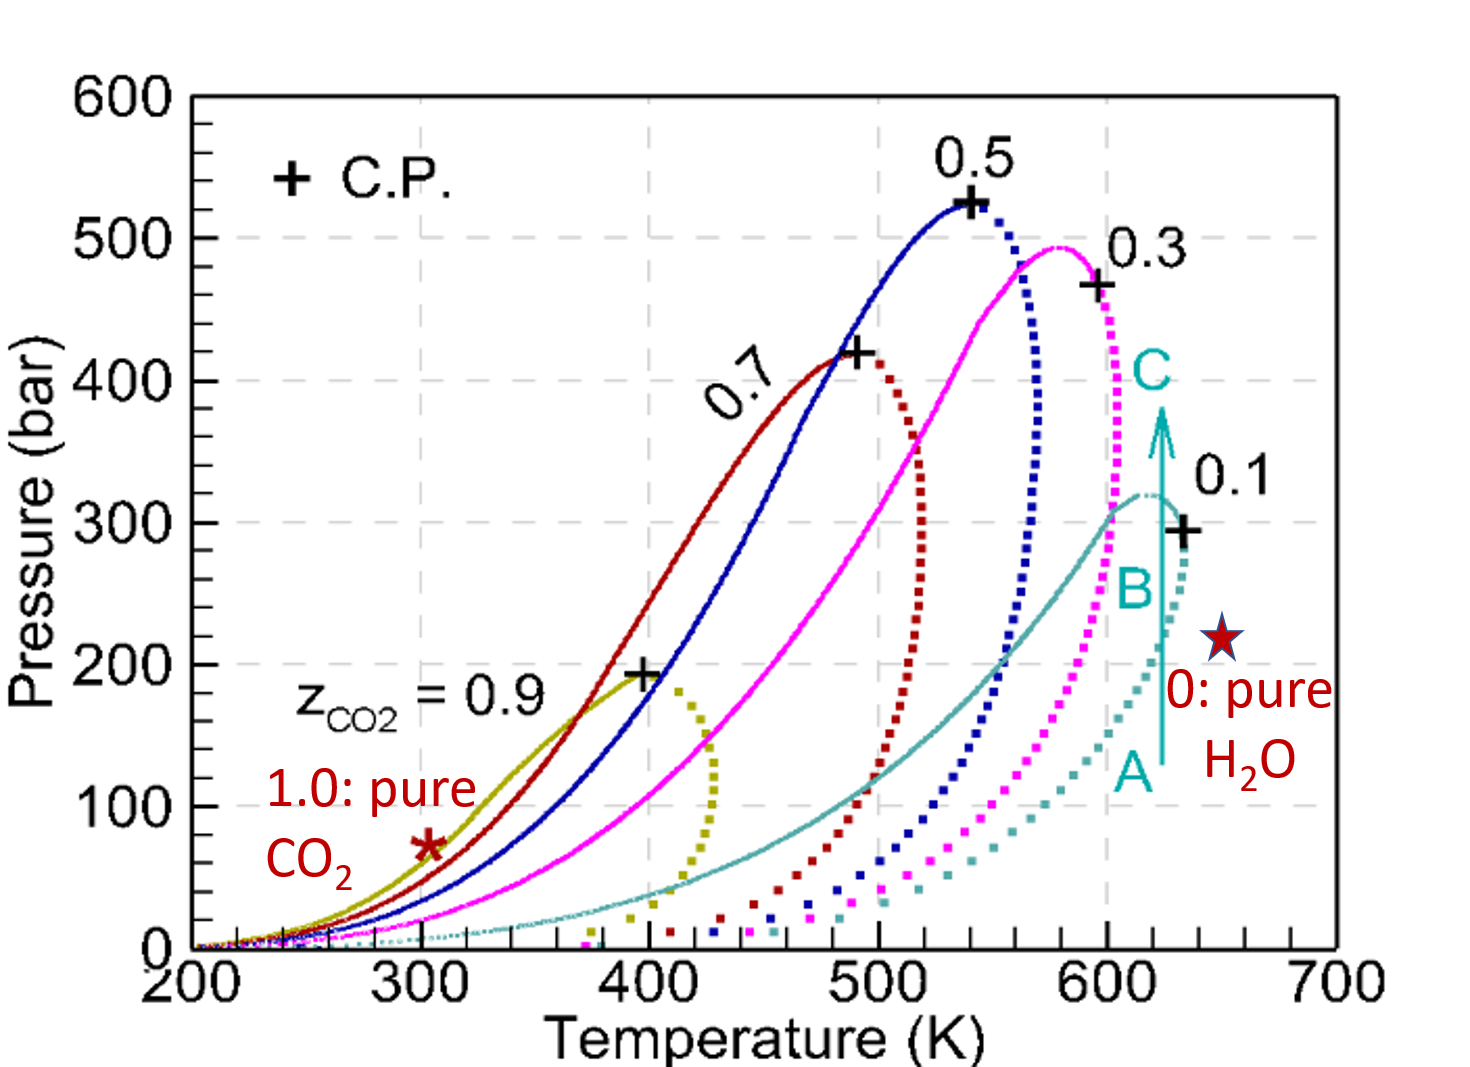
\includegraphics[width=0.5\linewidth]{phase_diagram_PT_CO2_H2O.png}
            %\caption{fig1}
            %\end{minipage}%
        }%
        \caption{Pressure-temperature phase boundaries and mixture critical points of \ce{CO2}/\ce{H2O} mixtures with different mole fraction values of \ce{CO2} (i.e., $z_{CO_2}$). Note the retrograde condensation behavior from A to B to C.}\label{v3}

    \end{figure}

As an example of two-component \ce{sCO2} systems, the pressure-temperature phase diagram of \ce{CO2}/\ce{H2O} mixtures is generated by the TPn flash solvers \cite{michelsen1982isothermal} (see details in the Supplementary Material of this article) and shown in Fig.~\ref{v3}. %The compressibility of this mixture with a feed of \ce{CO2}/\ce{H2O}=0.3/0.7 is shown in Fig.~\ref{v3}(b).
The mixture critical pressures can be significantly higher than the critical pressure of each individual component (i.e., pure \ce{CO2} and pure \ce{H2O}).
As a result, at conditions close to the critical point of pure \ce{CO2} (304.13 K, 73.78 bar), the \ce{CO2}/\ce{H2O} mixtures (with $\ge10\%$ \ce{H2O}) are in subcritical liquid phase. Therefore, a so-called ``supercritical \ce{CO2}'' system might be in a subcritical state due to the rise of mixture critical points caused by some impurities. In order to get a supercritical state for the \ce{CO2}/\ce{H2O} mixtures, the pressure and temperature need to be elevated about 100-200 K and 100-500 bar, respectively. %If the temperature and pressure are still close to those in the traditional closed \ce{sCO2} systems, the mixtures in the compressors of \ce{sCO2} gas turbine systems will be in liquid phase, which could cause erosion.
In addition, retrograde condensation behavior could occur in such systems. % Retrograde condensation behavior has been explained in Sec.~\ref{app:trad}.%: 
Specifically, when the subcritical gas (at Point A) is compressed into the subcritical two-phase zone, phase separation could occur, and the gas partially condenses into liquid (at Point B), but further compression makes the mixture go outside of the two-phase zone such that the liquid component (at point B) evaporates again (i.e., the so-called ``retrograde condensation") to Point C. Similar but the reverse process occurs during the expansion from Point C to Point A.
%\ce{CO2}/\ce{CH4} mixtures exist near the fuel injector in a \ce{sCO2} oxy-combustor. The mixtures with $z_{\ce{CO2}}$ from 0 to 1 are the jet-in-crossflow mixtures from the fuel injector to the end of the penetration length. Since \ce{sCO2} oxy-combustors always contain some water (e.g., the cooler cannot remove all water generated by the last cycle's combustion), it influences the thermodynamic state of the mixture. As a result, even the typical working conditions (100-300 or 400 bar, 300-1000 K) may overlap with the two-phase zone. Accordingly, this section investigates the influence of different levels of \ce{H2O} addition on the \ce{CO2}/\ce{CH4} mixture phase diagrams. %In the literature, the phase diagram as well as the tangent plane distance (TPD) method are commonly used to justify the phase state. %(??)Both the phase state and TPD are validated for single component, but are invalidated for multicomponent mixture because their values are affected by the feed, which is determined by the mixing process. 
As another example of two-component \ce{sCO2} systems, Figure~\ref{v5}(a) shows the thermodynamic states of \ce{CO2}/\ce{CH4} mixtures. Similar to the \ce{CO2}/\ce{H2O} mixtures in Fig.~\ref{v3}, the mixture critical pressures of \ce{CO2}/\ce{CH4} can also be higher than those of both pure \ce{CH4} and pure \ce{CO2}.

%With the help of \ce{CO2}, significant higher critical pressures can be obtained compared to typical gas turbine engines in Fig.~\ref{v4}(a). 

%However, the typical working conditions are still far away from the two-phase zones of all possible \ce{CO2}/\ce{CH4} mixture compositions. Thus the mixtures are always in supercritical gas-like states.

\begin{figure}[htb]
    \centering

    \subfigure{
        \begin{minipage}[t]{1\linewidth}
            \centering
            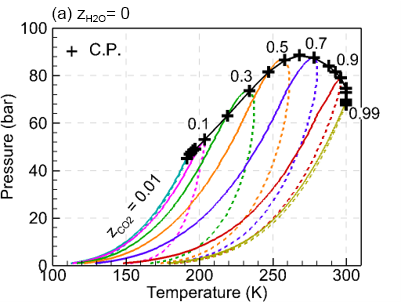
\includegraphics[width=0.45\linewidth]{phase_diagram_PT_CO2_CH4.png}
            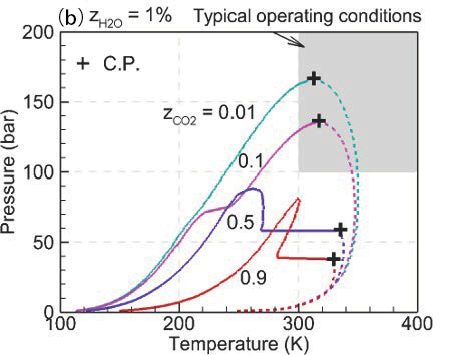
\includegraphics[width=0.45\linewidth]{phase_diagram_PT_CO2_CH4_1_H2O.png}
            %\caption{fig1}
        \end{minipage}%
    }%

    \subfigure{
        \begin{minipage}[t]{1\linewidth}
            \centering
            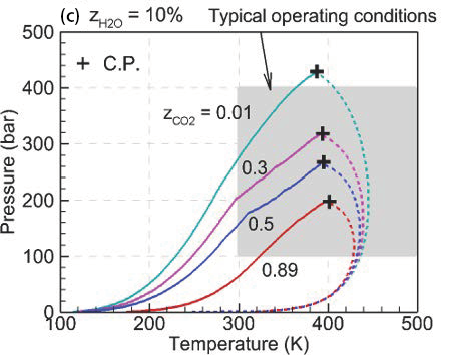
\includegraphics[width=0.45\linewidth]{phase_diagram_PT_CO2_CH4_10_H2O.png}
            %\caption{fig2}
        \end{minipage}%
    }%
    \caption{Effects of \ce{H2O} addition on the pressure-temperature phase boundaries and critical points of \ce{CO2}/\ce{CH4}/\ce{H2O} mixtures: (a) no \ce{H2O} addition; (b) 1\% \ce{H2O} addition; (c) 10\% \ce{H2O} addition.}
    \label{v5}
\end{figure}

As an example of three-component \ce{sCO2} systems, Figure~\ref{v5} shows the influence of different levels of \ce{H2O} addition on the \ce{CO2}/\ce{CH4}/\ce{H2O} mixture phase diagrams.
As shown in Fig.~\ref{v5}(b), even only 1\% of \ce{H2O} addition can increase the mixture critical point significantly. When the amount of \ce{CO2} is sufficiently small (e.g., $z_{CO_2}\leq0.1$), the mixture critical pressure can be larger than 100 bar. %make the two-phase zone enter the typical operating conditions if the amount of \ce{CO2} is sufficiently small (e.g., $z_{CO_2}\leq0.1$). But when there is a large amount of \ce{CO2} in the mixture (e.g., $z_{CO_2}\geq0.5$), the operating conditions could be purely supercritical and gas-like. Therefore, phase separation could occur near the fuel injector, but its region might be small.
As shown in Fig.~\ref{v5}(c), when $z_{H_2O}$ rises to 10\%, the mixture critical point increase even further. The mixture critical pressure can range from 200 to 400 bar.
The typical working condition range of \ce{sCO2} oxy-combustors (100-400 bar and $\ge300$ K) is indicated in Fig.~\ref{v5}. With \ce{H2O} addition, that working condition range overlaps with the subcritical two-phase zone, indicating that phase separation could occur.
%the operating conditions always intersect with the two-phase zone regardless of the amount of \ce{CO2} in the mixture. As a result, phase separation occurs through a large portion of the fuel jet until the temperature is sufficiently high.
Another typical three-component \ce{sCO2} systems are the \ce{CO2}/\ce{CH4}/\ce{O2} systems, which are investigated in Appendix~\ref{app:trad} and show similar retrograde condensation behavior as the \ce{CO2}/\ce{H2O} systems in Fig.~\ref{v3}.


\subsubsection{Influence of mixture critical point and phase change on the thermodynamic properties of the \ce{sCO2} systems}
\label{sec:results:combustor:phase}
The mixture critical point and phase change affect all mixture thermodynamic properties, because all of them are functions of reduced pressure ($p_r=p/p_c$) and reduced temperature ($T_r=T/T_c$), especially when the thermodynamic state is close to the critical point and/or deviates from ideal gas (typically high $p$ low $T$ conditions). %, as shown in Appendix~\ref{app:compressibility}). %Among these properties, the density, specific heats, thermal conductivity, mass diffusivity, speed of sound and internal energy are largely affected.

    %\comment{The previous section has shown that the typical working conditions of \ce{sCO2} oxy-combustors can encounter the two-phase zone, and hence phase separation can occur. But the influence of phase separation on the fluid properties is still unclear, which is investigated in this section.
    %This section investigates the influence of phase separation on the fluid properties.}

    %To avoid repeating the same information,

    %In oxy-combustors, the locations where \ce{CH4} and \ce{O2} have mixed but not yet reached an ignition or a flame are considered here. At such locations, the \ce{CO2} concentration is very high, so its concentration is assumed to be 90\%. Due to the cooler, the \ce{H2O} concentration is typically low in \ce{sCO2} combustors, so its concentration is assumed to be 1\%. Without loss of generality, the concentration of \ce{CH4} and \ce{O2} are both assumed to be 4.5\%.

     Figure~\ref{fig:PTdiagram_rho} shows the density of the mixture with and without phase separation. Comparing to the $z_{\ce{CO2}}=0.9$ curve in Fig.~\ref{v5}(b), it is seen that with the addition of \ce{O2}, the mixture critical pressure further rises from below 50 bar to approximately 350 bar. As a result, a significant part of the typical working conditions overlaps with the subcritical two-phase zone to trigger phase separation. By comparing Fig.~\ref{fig:PTdiagram_rho}(a) and (b), it is seen that at the relevant conditions of this work (i.e., 100-300 bar), phase separation only has a small influence on the density of this specific mixture. This indicates that the assumption of ``supercritical dense gas-like fluid" in Fig.~\ref{fig:PTdiagram_rho}(b) could result in a similar mixture density as the real subcritical two-phase mixture in Fig.~\ref{fig:PTdiagram_rho}(a) at the same thermodynamic condition.

    \begin{figure}[htb]
        \centering

        \subfigure{
            \begin{minipage}[t]{1\linewidth}
                \centering
                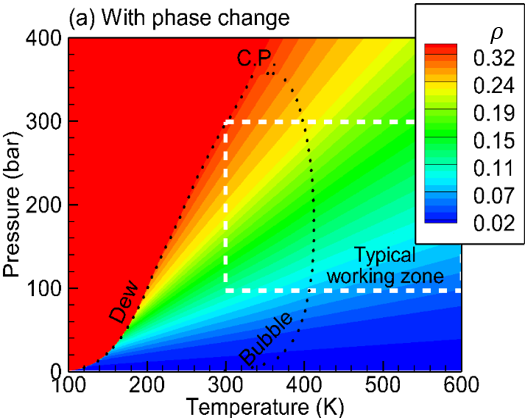
\includegraphics[width=0.45\linewidth]{rho_PT_VLE.png}
                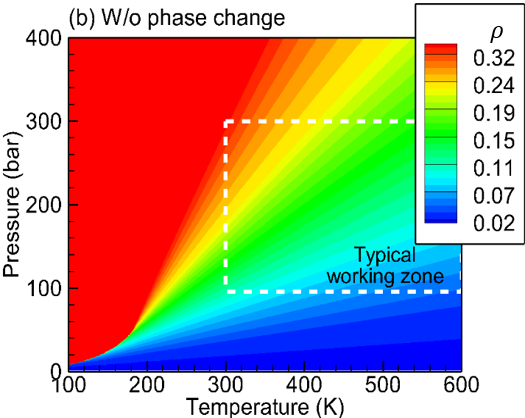
\includegraphics[width=0.45\linewidth]{rho_PT_noVLE.png}
                %\caption{fig1}
            \end{minipage}%
        }%

        \caption{Density ($\rho$) of \ce{CO2}/\ce{H2O}/\ce{CH4}/\ce{O2} mixture with an overall mole fraction of 0.9/0.01/0.045/0.045 in the pressure-temperature phase diagram: (a) with phase change (i.e., with VLE); (b) without phase change (i.e., without VLE).}
        \label{fig:PTdiagram_rho}
    \end{figure}

    In contrast, Figure~\ref{fig:PTdiagram_cp} shows that phase separation has a considerable influence on the isobaric heat capacity of the mixture. This could significantly affect the heating/evaporating timescale of the mixture and consequently, affect the ``effective" ignition delay in the cold ignition process.

    \begin{figure}[htb]
        \centering

        \subfigure{
            \begin{minipage}[t]{1\linewidth}
                \centering
                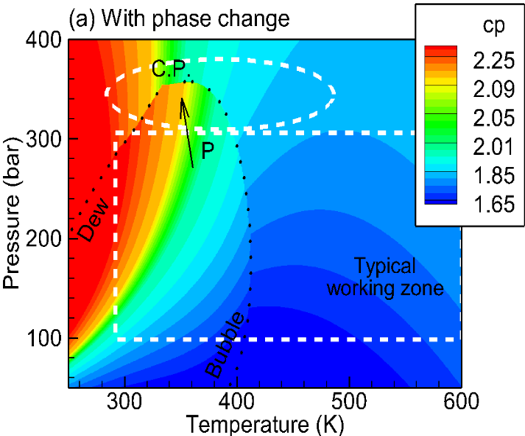
\includegraphics[width=0.45\linewidth]{cp_PT_VLE.png}
                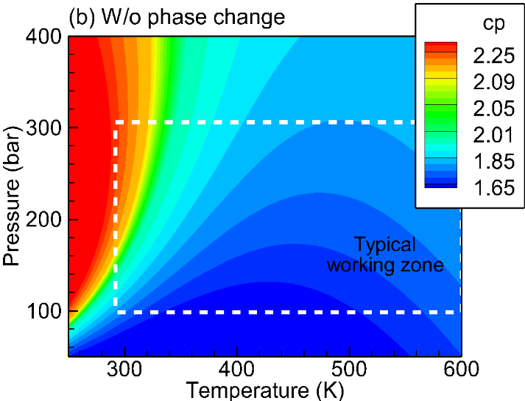
\includegraphics[width=0.48\linewidth]{cp_PT_noVLE.png}
                %\caption{fig1}
            \end{minipage}%
        }%

        \caption{Isobaric heat capacity ($c_p$) of \ce{CO2}/\ce{H2O}/\ce{CH4}/\ce{O2} mixture with an overall mole fraction of 0.9/0.01/0.045/0.045 in the pressure-temperature phase diagram: (a) with phase change (i.e., with VLE); (b) without phase change (i.e., without VLE).}
        \label{fig:PTdiagram_cp}
    \end{figure}


%\subsubsection{Subcritical and supercritical mixing and phase separation in \ce{sCO2} oxy-combustors}
%\label{sec:results:combustor:HPn}
\subsubsection{Isobaric and isenthalpic (HPn) mixing in the \ce{sCO2} systems: \ce{H2O}-induced low-T phase separation} \label{sec:results:combustor:HPn}
The previous analyses %for \ce{sCO2} oxy-combustors
are based on the pressure-temperature phase diagrams generated by the isothermal and isobaric (TPn) flash solver \cite{michelsen1982isothermal}.
%In real \ce{sCO2} oxy-combustors,
However, many real mixing processes follow the isobaric and isenthalpic (HPn) path \cite{serrano2018development}. Thus the real phase states should be determined based on the isenthalpic mixing process generated by the HPn flash solver \cite{michelsen1987multiphase}. Details of both TPn and HPn flash solvers are provided in Michelsen's works \cite{michelsen1982isothermal,michelsen1987multiphase} and the Supplementary Material of this article.
%, which was discussed in Sec.~\ref{thermo models}.
%All analyses above are based on temperature and pressure using TPn flash solver, but for isentropic mixing process, HPn flash is more suitable to describe phase split in mixing processes. 
%Here, we are going to analyze the isentropic mixing process in combustor using HPn flash result.

Based on Fig.~\ref{v7}, for the mixing between 300 K \ce{CH4} and 900 K \ce{CO2} without \ce{H2O}, it is in a supercritical gas-like state during the whole mixing process, which agrees with the observation from the pressure-temperature phase diagram in Fig.~\ref{v5}(a). Note that although not shown here, the same conclusion is observed when the ambient temperature of \ce{CO2} is below 700 K.
%This is confirmed by tangent plane distance (TPD) phase stability test \citep{michelsen1982isothermal}, which is a number of numerical methods for stability analysis based on Gibbs’ tangent plane criterion, in Fig.~\ref{v7} as expected.
\begin{figure}[htb]
    \begin{center}
        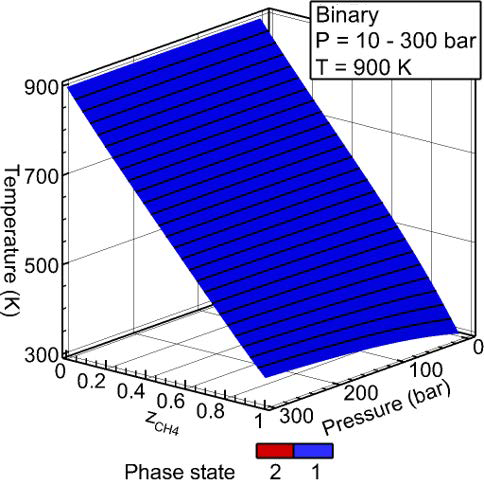
\includegraphics[width=0.4\linewidth]{mixing_temperature_CO2_CH4.png}
    \end{center}
    \caption{Equilibrium mixing temperature $T_{eq}$ for the mixing between 900 K \ce{CO2} and 300 K \ce{CH4}: the pressure is in the range of 10 – 300 bar, and the overall mole fraction of \ce{CH4} is in the range of 0.01 – 0.99. Red: two-phase zone; blue: single-phase zone.}
    \label{v7}
\end{figure}

As shown in Fig.~\ref{v8}, with the help of \ce{H2O}, the subcritical two-phase zone can start to play an important role. %For the mixture of \ce{CO2}/\ce{CH4}/\ce{H2O}%, superimposing the true adiabatic mixing temperature (TAMT) is on the mixture critical locus line, the two-phase region can be easily determined. 
For the mixing between \ce{CH4} (300 K) and \ce{CO2}/\ce{H2O} mixture, if the ambient temperature (i.e., the temperature of \ce{CO2}/\ce{H2O} mixture) is lower than 700 K (i.e., Fig.~\ref{v8} (a-b)), the mixture can pass through the subcritical two-phase zone. The area of the two-phase zone increases as the pressure increases from 100 bar to 400 bar. When the ambient temperature reaches 900 K in Fig.~\ref{v8}(c), the mixing process does not pass the subcritical two-phase zone, so there is no more phase separation. Hence, for \ce{sCO2} systems with low temperatures (e.g., 700 K or lower), \ce{H2O} can cause phase separation. But for high-temperature \ce{sCO2} systems (e.g., 900 K or higher), phase separation cannot happen.  %\comment{But this ambient temperature is possible only near the fuel injectors and too low for the downstream locations of real \ce{sCO2} oxy-combustors. Based on the literature \citep{delimont2017direct}, the auto-ignition occurred at high concentrations of \ce{CO2} at least 900 K (i.e., Fig.~\ref{v8}(c)). For the lowest auto-ignition temperature (i.e., 900 K) and highest pressure (i.e., 400 bar), the mixing process still does not pass the two-phase zone, so there is no phase separation.}
\begin{figure}[htb]
    \centering
    \subfigure{
        \begin{minipage}[t]{1\linewidth}
            \centering
            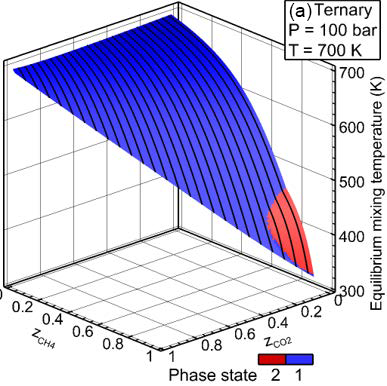
\includegraphics[width=0.32\linewidth]{mixing_temperature_CO2_CH4_H2O_100bar_700k.png}
            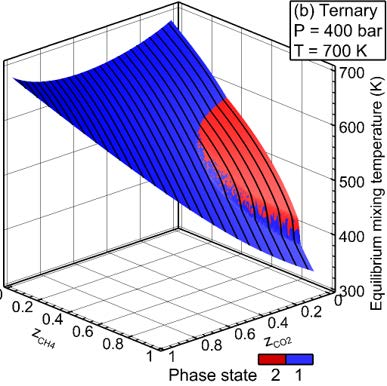
\includegraphics[width=0.32\linewidth]{mixing_temperature_CO2_CH4_H2O_400bar_700k.png}
            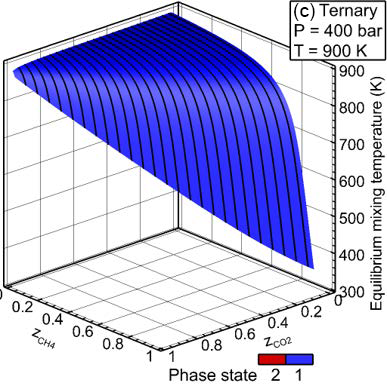
\includegraphics[width=0.32\linewidth]{mixing_temperature_CO2_CH4_H2O_400bar_900k.png}
            %\caption{fig1}
        \end{minipage}%
    }%

    \caption{Equilibrium mixing temperature $T_{eq}$ for the mixing between \ce{CH4} at 300 K and \ce{CO2}/\ce{H2O} mixture at the ambient pressure and temperature of (a) 100 bar and 700 K; (b) 400 bar and 700 K; and (c) 400 bar and 900 K. Red: two-phase zone; blue: single-phase zone.}
    \label{v8}
\end{figure}


\subsection{1D simulation of a laminar premixed \ce{sCO2} shock tube: condensation driven by an expansion wave}
\label{sec:results:ShockTube}
%Compression and expansion processes occur in the \ce{sCO2} compressors and turbines. 
Since semi-closed \ce{sCO2} systems contain both compression and expansion processes (e.g., in the compressor stage and turbine stage, respectively), it is important to study the compression and expansion effects on real fluid and VLE. Shock tube is the simplest configuration to contain both compression and expansion processes, and hence is ideal to study those effects. In addition, \ce{sCO2} shock tube is a common experimental facility to study semi-closed \ce{sCO2} systems, whose designs require insights from computational studies. 
A shock tube case of a \ce{CO2}/\ce{H2O} mixture is tested at high-pressure conditions,
%relevant to \ce{sCO2} gas turbine systems, 
which is used to compare different thermodynamics models. The initial condition is set close to the phase boundary to show the interaction between shock wave and phase change.  %, and also help understand the compression and expansion processes.
%In order to mimic the compression process in \ce{sCO2} compressors and expansion process in \ce{sCO2} turbines, a shock tube case of a \ce{CO2}/\ce{H2O} mixture is tested, which includes a compression shock wave and an expansion wave. 
%The Mach number of flow in this shock tube is 1.25, which indicates the need of the transonic version of the PIMPLE algorithm (see Appendix~\ref{App:gp}) to handle the compressibility of relatively large Mach number flows. 
As shown in Appendix~\ref{App:vali:CFD}, the CFD solver has been validated and verified by other shock tube cases. The initial condition of the current test case is shown in Table~\ref{conditions}.
\begin{table}[htbp]

    \begin{center}
        \begin{minipage}{0.8\textwidth}
            \caption{Initial condition of a shock tube with \ce{CO2}/\ce{H2O} mixture. Domain length: 0.1 m; membrane location: 0.05 m}\label{conditions}
            \begin{center}
                \begin{tabular}{@{}lllll@{}} %\hline
                    \toprule
                               & $P$ (bar) & $T$ (K) & $x_{\rm CO_2}$ & $x_{\rm H_2O}$ \\ %\hline
                    \midrule
                    left side  & 230       & 500     & 0.7            & 0.3            \\ %\hline
                    right side & 100       & 550     & 0.7            & 0.3            \\ %\hline
                    \bottomrule
                \end{tabular}
            \end{center}
        \end{minipage}
    \end{center}

\end{table}

\begin{figure}[htb]
    \centering
    \subfigure{
        \begin{minipage}[t]{1\linewidth}
            \centering
            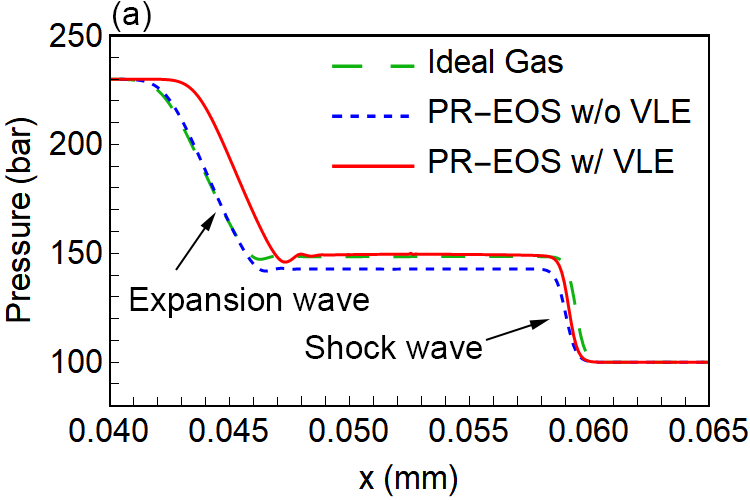
\includegraphics[width=0.45\linewidth]{shock_tube_p.png}
            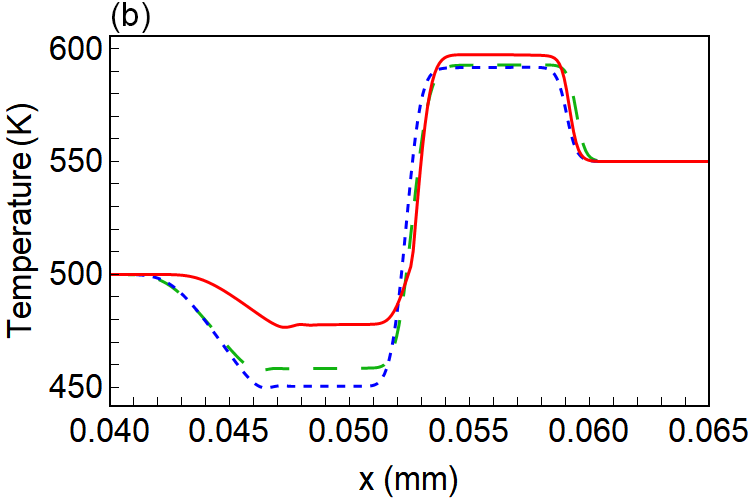
\includegraphics[width=0.45\linewidth]{shock_tube_T.png}
            %\caption{fig1}
        \end{minipage}%
    }\\
    %#\subfigure{\begin{minipage}[t]{1\linewidth}
    %\centering
    %\includegraphics[width=1.5in]{st/stt1.png}
    %\caption{fig2}
    %\end{minipage}%
    %}
    \subfigure{
        \begin{minipage}[t]{1\linewidth}
            \centering
            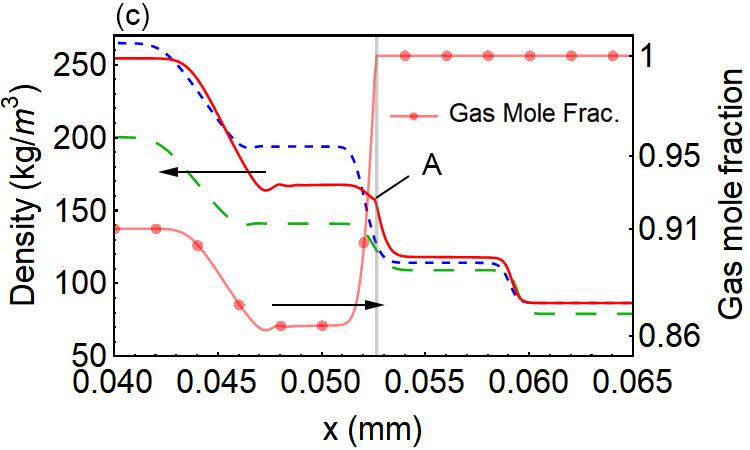
\includegraphics[width=0.50\linewidth]{shock_tube_rho.png}
            %\caption{fig2}
        \end{minipage}%
    }%
    %\subfigure{
    %\begin{minipage}[t]{1\linewidth}
    %\centering
    %\includegraphics[width=2in]{st/stvf_rho.png}
    %\caption{fig2}
    %\end{minipage}%
    %}%
    \caption{Simulation results of a shock tube with \ce{CO2}/\ce{H2O} mixture, at $t=2\times10^{-8}s$: (a) pressure; (b) temperature; (c) density and gas mole fraction.}
    \label{v9}
\end{figure}

To show the importance of real-fluid EOS and VLE models in CFD simulations, three models are used and compared:
\begin{itemize}
    \item ideal gas model;
    \item real-fluid model (PR-EOS) without phase change (i.e., without VLE);
    \item real-fluid model (PR-EOS) with phase change (i.e., with VLE).
\end{itemize} %( From Fig.\ref{v9}, expansion wave speed of phase change result is smaller which is caused by the different sound speed of liquid mixture.)
From the pressure plot in Fig.~\ref{v9}(a), it is apparent that the expansion wave in the PR-EOS model with VLE propagates slower, which is due to lower sound speed (with VLE: 312-323 m/s; without VLE: 363-378 m/s. The VLE sound speed is calculated based on the formula in Tudisco and Menon \cite{tudisco2020analytical}). The phase equilibrium includes thermal equilibrium, mechanical equilibrium, and chemical equilibrium. In an isentropic process (i.e., $dS=0$), when volume decreases (i.e., for a given $dV<0$), these equilibria mitigate the pressure rise to minimize the total energy $E$ and hence minimize the total energy rise $(dE = -pdV + TdS)$. Consequently, with the same $\Delta\rho$, phase equilibrium makes $p$ and hence the pressure rise $\Delta p$ smaller than those without VLE. According to the formula of sounds speed $c=\sqrt{\Big(\frac{\partial p}{\partial \rho}\Big)_s}$, VLE causes the drop of sound speed.
%Specifically, in the isentropic process, at a change in density, the pressure change is reduced by phase change, and hence sound speed $c=\sqrt{\Big(\frac{\partial p}{\partial \rho}\Big)_s}$ is smaller. In contrast, the mixture in the compression shock wave is in a pure gas phase due to the higher temperature. Thus, the shock wave speed is not affected by phase change. %, and the post-compressor mixture should be in a pure gas phase.
In Fig.~\ref{v9}(b), because phase change is taken into account, latent heat is released when vapor partially condenses during the expansion wave propagation, which reduces the temperature reduction and makes PR-EOS with VLE have the highest temperature. In Fig.~\ref{v9}(c), the three models show evident differences in density prediction. Specifically, compared to the real-fluid models (PR-EOS), the ideal gas model underestimates the gas density. The effect of the phase change (i.e., VLE) increases the temperature in the expansion wave and hence reduces the density there. The gas mole fraction, predicted by the real-fluid model with phase change (i.e., with VLE) at different positions, indicates that the mixture is partially condensed after the expansion wave. Also, a sharp bend (point A) in the density line only exists in the prediction from the PR-EOS model with VLE, which corresponds to the location where the mixture starts to condense.

In summary, the real fluid model integrated with VLE can capture more physics caused by phase change. %including: the propagation of expansion waves slows down, and temperature jump is mitigated.
The results show that expansion waves can trigger significant condensation in premixed \ce{sCO2} systems, and the latent heat of the condensation can change the temperature and density fields in the systems. Moreover, the speed of the expansion wave is reduced.

\subsection{3D LES of turbulent jet-in-crossflows in the \ce{sCO2} systems: mixing-driven phase separation}
\label{sec:results:JICF}
To understand the mixing-driven phase separation in the \ce{sCO2} systems (e.g., the fuel and oxidizer injections in \ce{sCO2} oxy-combustors), large-eddy simulations (LES) of turbulent jet-in-crossflows are conducted. As shown in Appendix~\ref{App:vali:CFD}, the CFD solver based on the PIMPLE algorithm has been validated by another turbulent jet-in-crossflow case. %\comment{In the current case, pure \ce{O2} and \ce{CH4} are used to represent the oxidizer and fuel, respectively.}
In each simulation, cold (300 K) \ce{O2} or \ce{CH4} is injected from the nozzle at the bottom into hot (500 K or 700 K) \ce{CO2} which contains a small amount of \ce{H2O} (10\% or 20\%). %\comment{to represent the \ce{H2O} generated by the combustion of the last cycle. The existing technology can achieve a \ce{CO2} mole fraction of 96\% in the \ce{sCO2} oxy-combustor \cite{mcclung2015high}. The mole fraction of \ce{H2O} can be 4\% or larger. Here, exaggerated values of 20\% and 10\% \ce{H2O} are used for simulation to show phase separation better.} 

Auto-ignition simulations at a constant pressure of 300 bar are conducted using Cantera \cite{goodwin2009cantera} with GRI-Mech 3.0 \cite{smith1999gri} as the chemical mechanism. Figure~\ref{JICFautoig} shows that at 700 K the ignition delay is about 20 s, but the time scales of the mixing and phase separation processes of the jet-in-crossflow in this study are less than 1 ms. Moreover, the injected \ce{O2} and \ce{CH4} are at 300 K, which makes it difficult to have any obvious chemical effect. For these reasons, chemical reactions do not need to be considered at the conditions of this study.

More details about settings, geometry, and mesh are shown in Table~\ref{JICFconditions} and Fig.~\ref{JICFg}. 
The mesh in the simulation contains 17.5M cells in total. The integral length scale $l_0$ is estimated using a Reynolds-averaged Navier–Stokes (RANS) simulation. $l_0\approx24 \rm{\mu m}$ in the interested region (0.4 cm $< x <$ 1.5 cm). The mesh in the interested region is refined to make sure $\Delta<l_0/5$, where $\Delta$ is the grid size and $\Delta \approx 3 \rm{\mu m}$. When the above condition is satisfied, about 80\% turbulent kinetic energy can be resolved by the mesh (the well-accepted criterion for LES resolution) \cite{gerasimov2016quick}, and hence the mesh resolution is high enough for LES \cite{pope2004ten}. Subgrid-scale (SGS) stress tensor is evaluated using the Smagorinsky model \cite{smagorinsky1963general}.  Since the VLE-based CFD of high-pressure multiphase flows is relatively new (more precisely, less than a decade), there is no investigation on the SGS mixing models of filtered VLE equations. Even the SGS mixing models for filtered real-fluid EOS are still not mature \cite{unnikrishnan2017subgrid,unnikrishnan2021subgrid}. %These models are necessary for the LES prediction of transcritical fluid flows, and hence need to be better investigated. 
In this work, due to the limitations of the state-of-the-art, we do not consider the SGS terms of filtered VLE equations and filtered real-fluid EOS but will investigate them in the future. % and only qualitatively investigate the mixing and phase separation in \ce{sCO2} gas turbine systems.} 

\begin{table}[htb]

    
    \begin{minipage}{0.9\textwidth}
        \caption{Injection nozzle and inflow conditions of the turbulent jet-in-crossflows.}    \label{JICFconditions}

        \begin{center}
            \begin{tabular}{@{}lllll@{}}% \hline
                \toprule
                $p$ (bar) & $T_{\rm{nozzle}}$ (K) & $T_{\rm{inflow}}$ (K) & $U_{\rm{nozzle}}$ (m/s) & $x_{\ce{H2O}}$ \\ %\hline
                \midrule
                300       & 300                   & 500 or 700            & 300                     & 0.2 or 0.1     \\%\hline
                \bottomrule
            \end{tabular}
        \end{center}
    \end{minipage}

\end{table}
\begin{figure}[htb]
    \centering
    \subfigure{
        \centering
        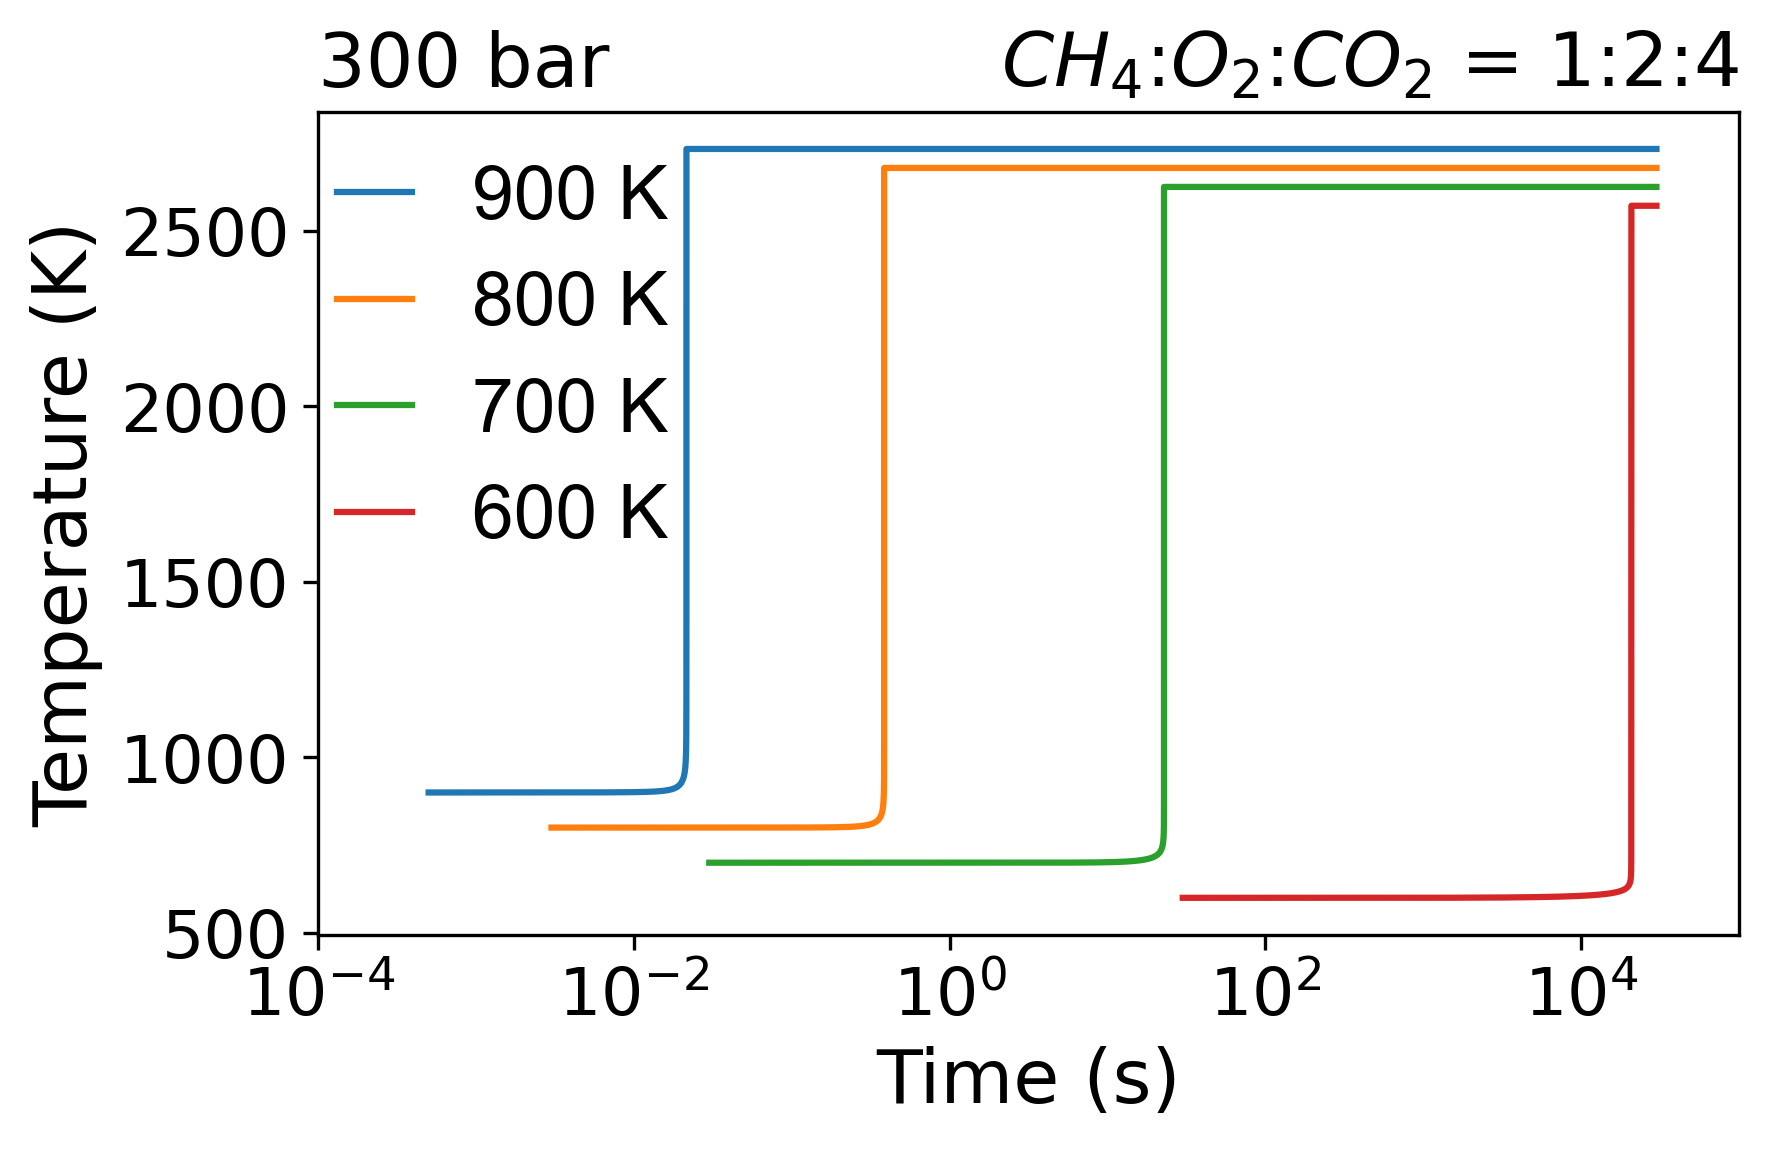
\includegraphics[width=0.6\linewidth]{autoig.png}
    }
    \caption{Temperature vs. Time plot: auto-ignition of \ce{CH4}/\ce{O2}/\ce{CO2} system at a constant pressure of 300 bar. \ce{CH4}:\ce{O2}:\ce{CO2} = 1:2:4, by mole.}
    \label{JICFautoig}
\end{figure}
\begin{figure}[htb]
    \centering
    \subfigure{
        \centering
        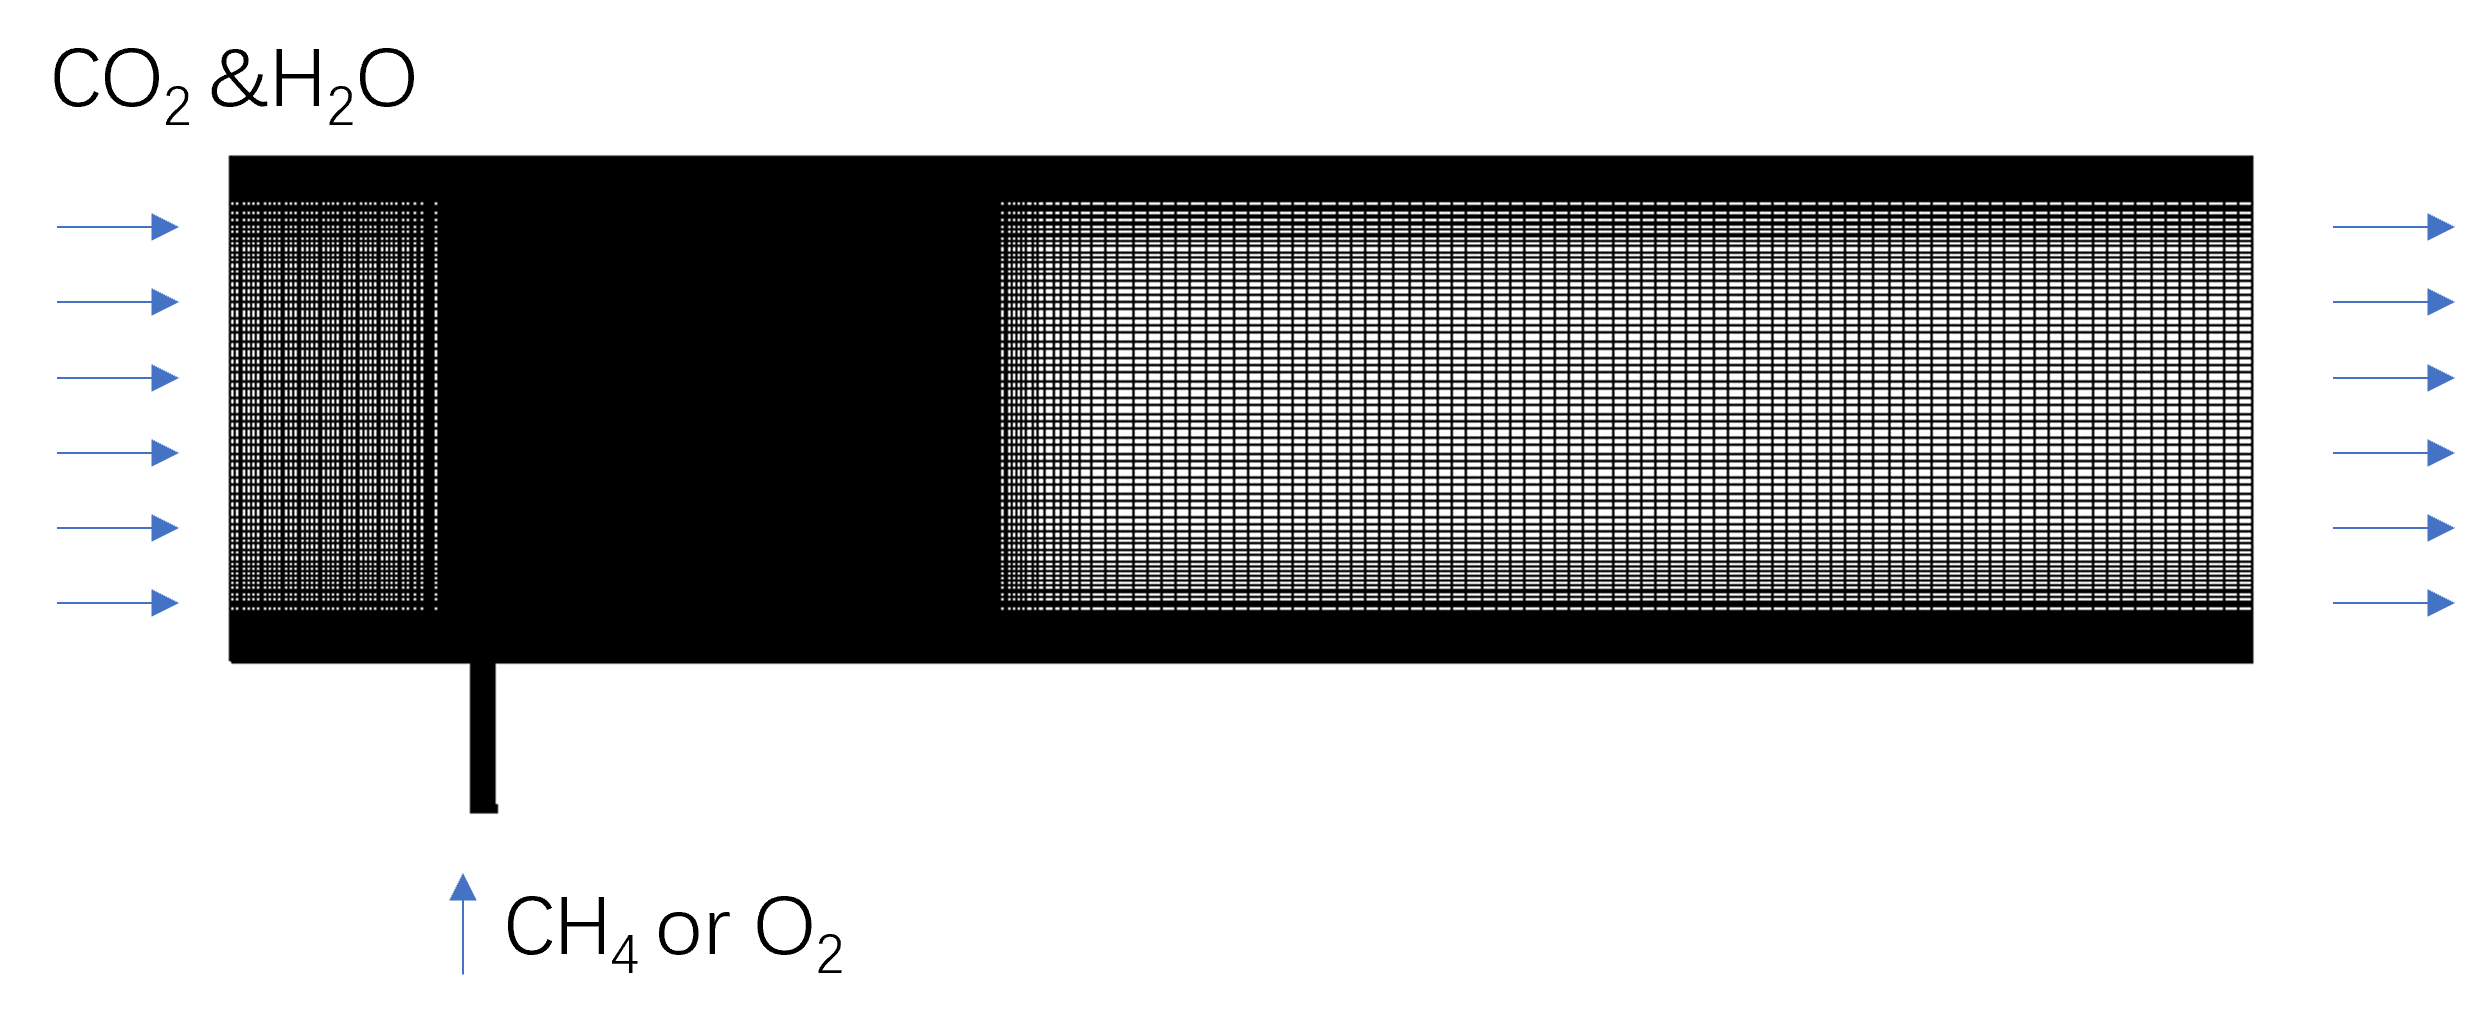
\includegraphics[width=0.6\linewidth]{fg2.png}
        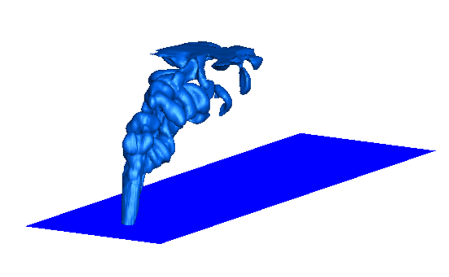
\includegraphics[width=0.4\linewidth]{JICF_schematic.png}
    }
    \caption{Computational mesh and geometry of the turbulent jet-in-crossflows, and iso-suface of \ce{CO2} mole fraction.}
    \label{JICFg}
\end{figure}

Figure~\ref{JICFr}(a-c) shows the results of \ce{O2} injection case. Near the injection nozzle, the cold \ce{O2} is mixed with the hot \ce{CO2}/\ce{H2O} mixture: \ce{O2} concentration keeps high as shown in Fig.~\ref{JICFr}(a), and temperature keeps low as shown in Fig.~\ref{JICFr}(b). In almost the same region, phase separation occurs as shown in Fig.~\ref{JICFr}(c). The cold \ce{O2} is in a supercritical gas-like state, and the hot \ce{CO2}/\ce{H2O} mixture is in the gas phase before they are mixed. However, the temperature of the injected \ce{O2} is low enough to let the gaseous \ce{H2O} in the working medium (i.e., the \ce{CO2}/\ce{H2O} mixture) partially condense (i.e., the mixture enters the subcritical two-phase zone). %After injecting \ce{O2} into the domain, the mixing process reduces the temperature of the mixture containing \ce{H2O}, and then the mixture partially condensed. 
With the mixing process proceeding, the low-temperature \ce{O2} is diluted, and the mixture temperature goes up to the initial temperature of the \ce{CO2}/\ce{H2O} mixture (i.e., the ambient temperature). The small amount of \ce{H2O} in liquid phase quickly evaporate back to the gas phase. Hence, phase separation only appears near the injection nozzle, which agrees with the 0D thermodynamics analysis in Sec.~\ref{sec:results:combustor:H2O}. A similar phenomenon is also observed in the \ce{CH4} injection case, as shown in Fig.~\ref{JICFr}(d).  with Fig.~\ref{JICFr}(d), the jet in Fig.~\ref{JICFr}(c) bends less, and has stronger breakup, which is due to different density ratio $r=\rho_{jet}/\rho_{\infty}$ where $\rho_{\infty}$ is the density of the working medium (i.e., the \ce{CO2}/\ce{H2O} mixture) and $\rho_{jet}$ is the density of the jet fluid from the injection nozzle. \ce{O2} jet has higher density ratio ($r=1.39$ from the data) than \ce{CH4} jet ($r=0.66$ from the data). The jet with higher density ratio trigger stronger breakup, which was also reported in Rachford et al. \cite{tretola2021effect}.

\begin{figure}[htb]
    \centering
    \subfigure{
        \centering
        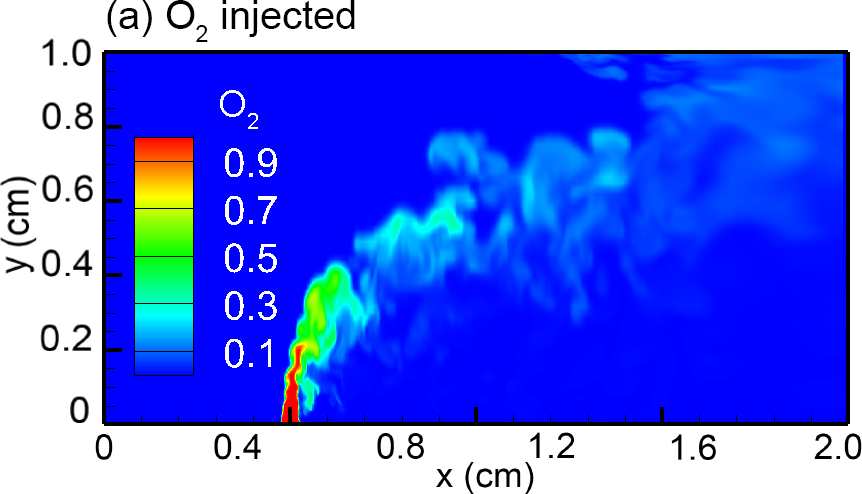
\includegraphics[width=0.45\linewidth]{1a_ps.png}
        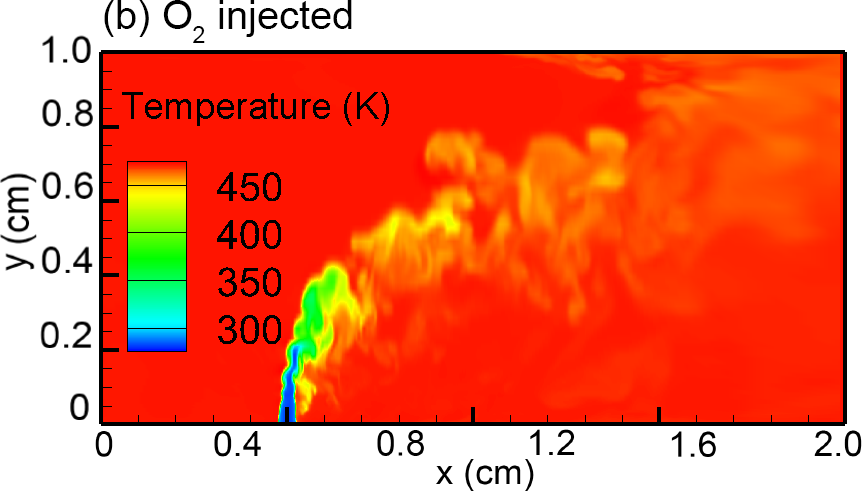
\includegraphics[width=0.45\linewidth]{1b_ps.png}
    }

    \subfigure{
        \centering
        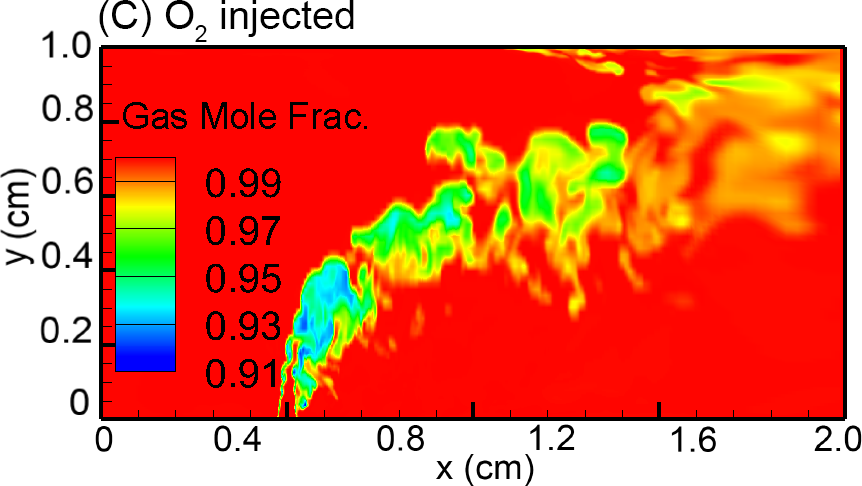
\includegraphics[width=0.45\linewidth]{1c_ps.png}
        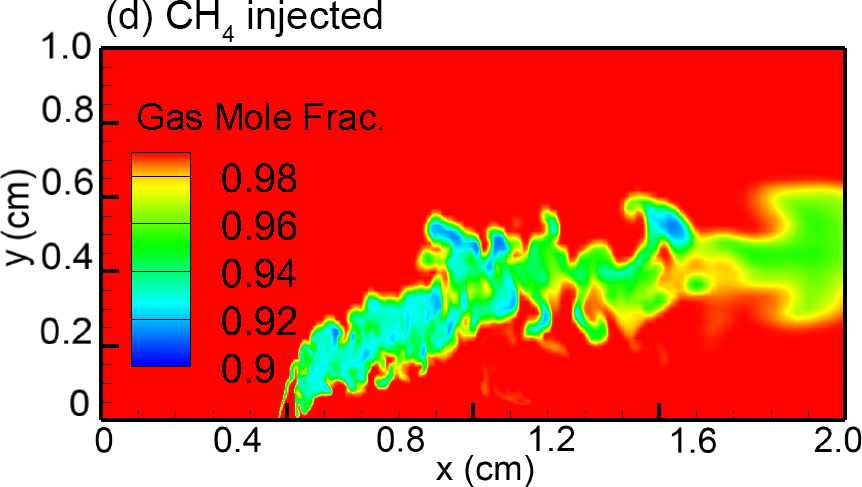
\includegraphics[width=0.45\linewidth]{1d_ps.png}
    }
    \caption{LES of turbulent jet-in-crossflows (ambient temperature is 500 K, and the \ce{CO2}/\ce{H2O} mixture has 20\% \ce{H2O}): (a) mole fraction of \ce{O2} (\ce{O2} is injected); (b) mixture temperature (\ce{O2} is injected); (c) mole fraction of vapor (gas) phase (\ce{O2} is injected); (d) mole fraction of vapor (gas) phase (\ce{CH4} is injected).}
    \label{JICFr}
\end{figure}

It is worth noting that the phase separation condition is sensitive to the variation of ambient temperature. Here, two more simulations for both \ce{CH4} and \ce{O2} injections are conducted at 700 K ambient temperature. The gas fraction distributions of both cases are shown in Fig.~\ref{JICF700}. The phase separation phenomenon becomes much weaker in these two cases: the phase separation region and its gas mole fraction become much smaller. As a result, only a small portion of the mixture condenses and quickly evaporates back to the gas phase.

\begin{figure}[htb]
    \centering
    \subfigure{
        \centering
        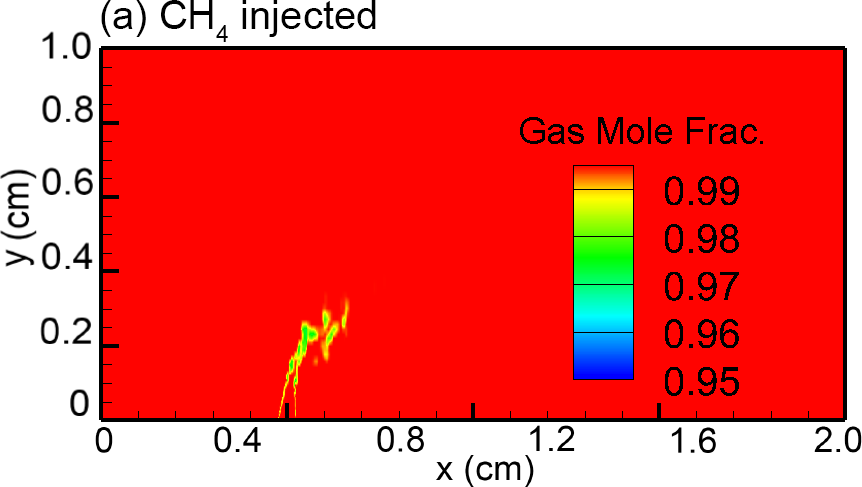
\includegraphics[width=0.45\linewidth]{2a_ps.png}
        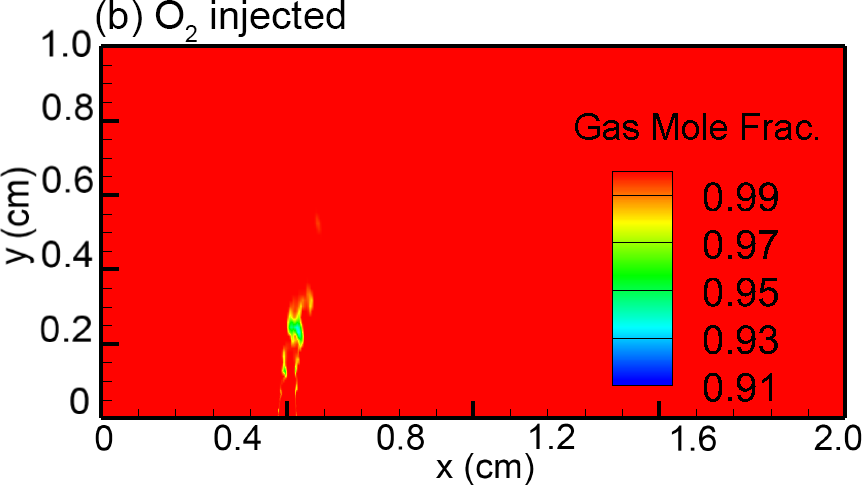
\includegraphics[width=0.45\linewidth]{2b_ps.png}
    }
    \caption{LES of turbulent jet-in-crossflows (ambient temperature is 700K, the \ce{CO2}/\ce{H2O} mixture has 20\% \ce{H2O}): (a) \ce{CH4} is injected; (b) \ce{O2} is injected.}
    \label{JICF700}
\end{figure}

A better understanding of the mixing process and the influence of temperature can be obtained by the thermodynamics analysis of the LES data. In Fig.~\ref{JICFT}, subcritical two-phase and gas-phase regions are colored grey and white, respectively. The phase boundary shown in the plot is at 300 bar. Although the pressure varies in the flow field, the range (289 - 307 bar) is relatively small, which has almost no effect on phase boundaries, as shown in Fig.~\ref{JICFTX}. Hence the phase boundary at 300 bar is a good representation of the boundaries of the system.  The dots are the local thermodynamic states encountered in the LES, which form a curve (i.e., mixing trajectory) to connect the thermodynamic states of the injected fluid and the ambient \ce{CO2}/\ce{H2O} mixture. Since the dew point of \ce{CO2} mixed with 20\% \ce{H2O} is about 500 K, when the ambient temperature is 500 K, the mixing trajectory (green dots) is almost entirely inside the subcritical two-phase zone. When the ambient temperature increases to 700 K, one end of the trajectory of thermodynamic states moves upward, which can be seen clearly from the red dots in Fig.~\ref{JICFT}. As a result, only a small portion of the curve stays inside the subcritical two-phase zone, and phase separation can be observed only in a small region. The isenthalpic mixing lines are also marked in Fig.~\ref{JICFT} to compare with the actual mixing trajectories. The difference between \ce{CH4} injection and \ce{O2} injection can be seen from the comparison between Fig.~\ref{JICFT}(a) and Fig.~\ref{JICFT}(b). For the scenarios with \ce{CH4} injection (Fig.~\ref{JICFT}(a)), at 500 K ambient temperature, the actual mixing trajectories almost overlaps with the isenthalpic lines, which is caused by weak thermal conduction; but at 700 K ambient temperature, larger temperature difference trigger stronger thermal conduction to raise the temperature, and hence the mixing temperature is mostly higher than the isenthalpic mixing temperature. %For the scenarios with \ce{O2} injection (Fig.~\ref{JICFT}(b)), the flow has strong mass diffusion effect. 
%the strong mass diffusion effect can be seen at 700 K ambient temperature, but the \ce{O2} scenarios have more significant mass diffusion effect, which enhances the thermal conduction of both the hot \ce{CO2}/\ce{H2O} mixture and the cold injected \ce{O2}. 
%Hence, the thermodynamic state points (red and green dots of mixing trajectories) of \ce{O2} scenarios are more dispersed than the \ce{CH4} scenarios. 
Compared with Fig.~\ref{JICFT}(a), the points in Fig.~\ref{JICFT}(b) are more dispersed, which is caused by higher density ratio (i.e., $r_{\ce{O2}}=2.4$ is higher than $r_{\ce{CH4}}=1.2$). Higher density ratio triggers stronger breakup, which enhances thermal conduction. Hence, more points deviate from the isenthalpic line.
Although the properties of \ce{CH4} and \ce{O2} affect the dispersion of thermodynamic state points, they do not significantly affect the phase boundaries and the area of the phase separation region in the physical space.

\begin{figure}[htb]
    \centering
    \subfigure{
        \centering
        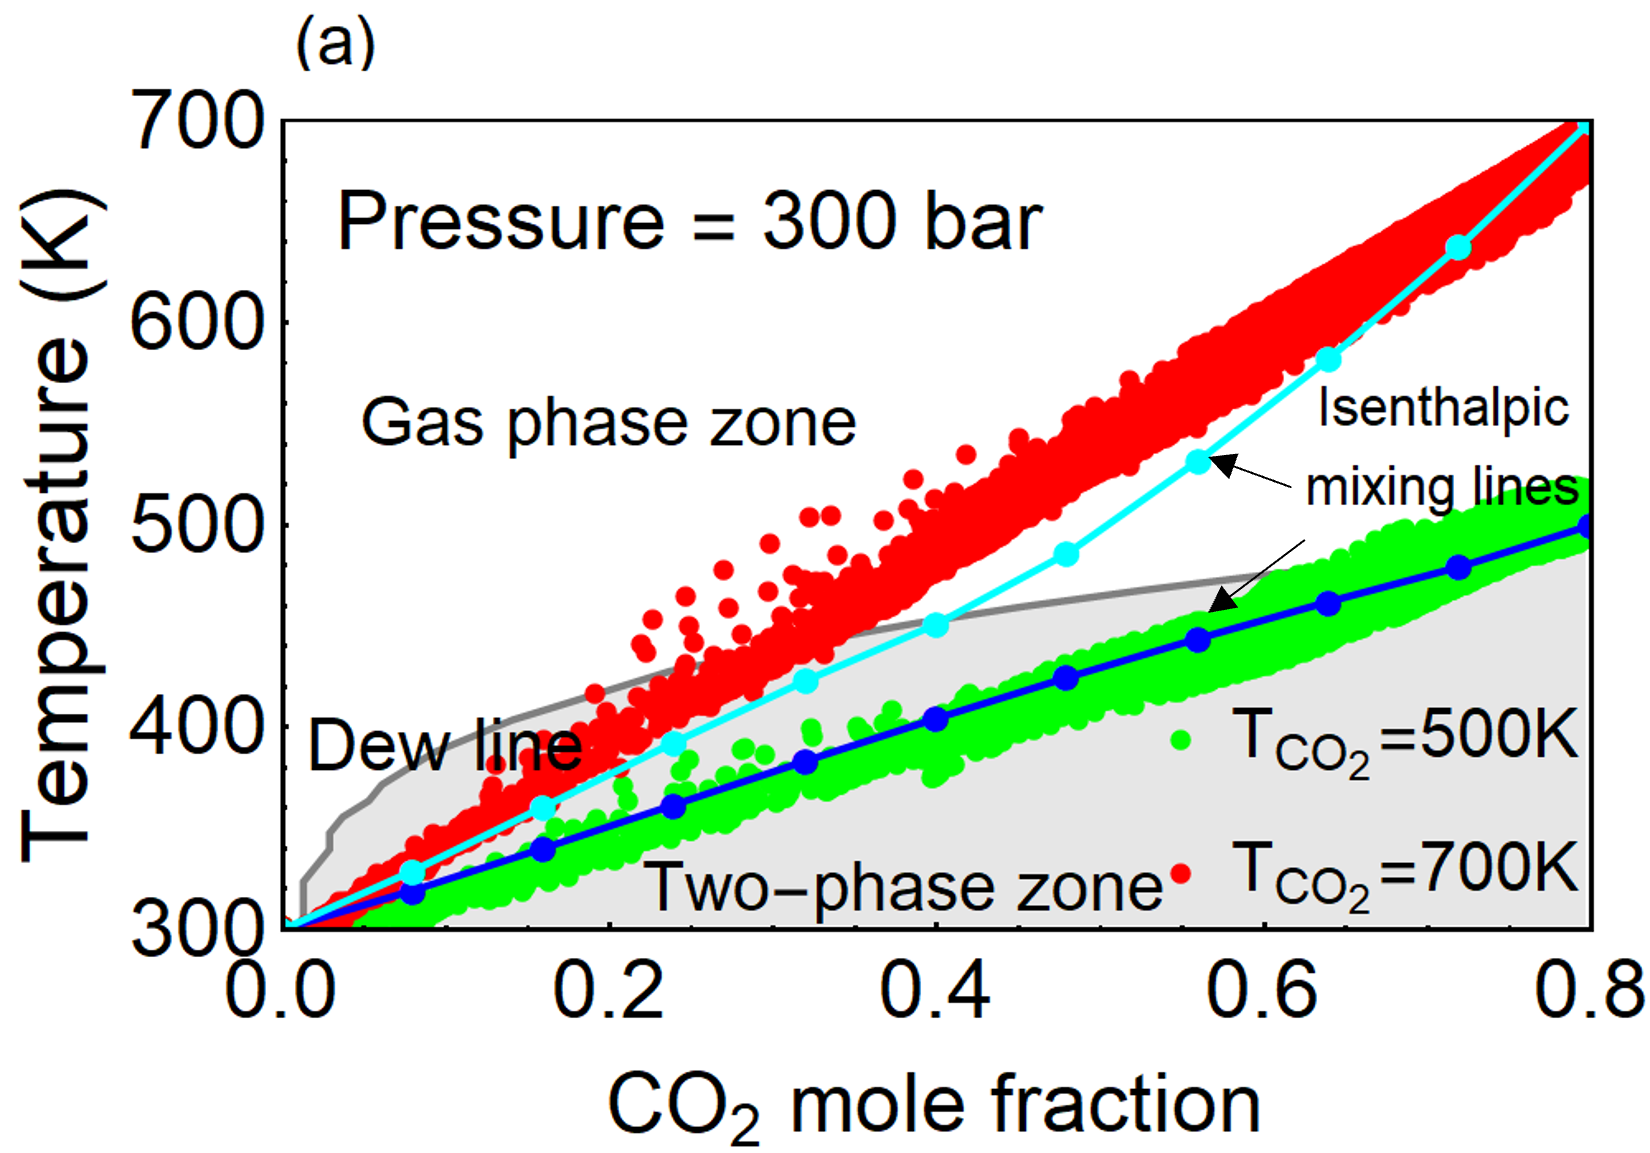
\includegraphics[width=0.45\linewidth]{Ccf_n_u_v2_flow_c.png}
        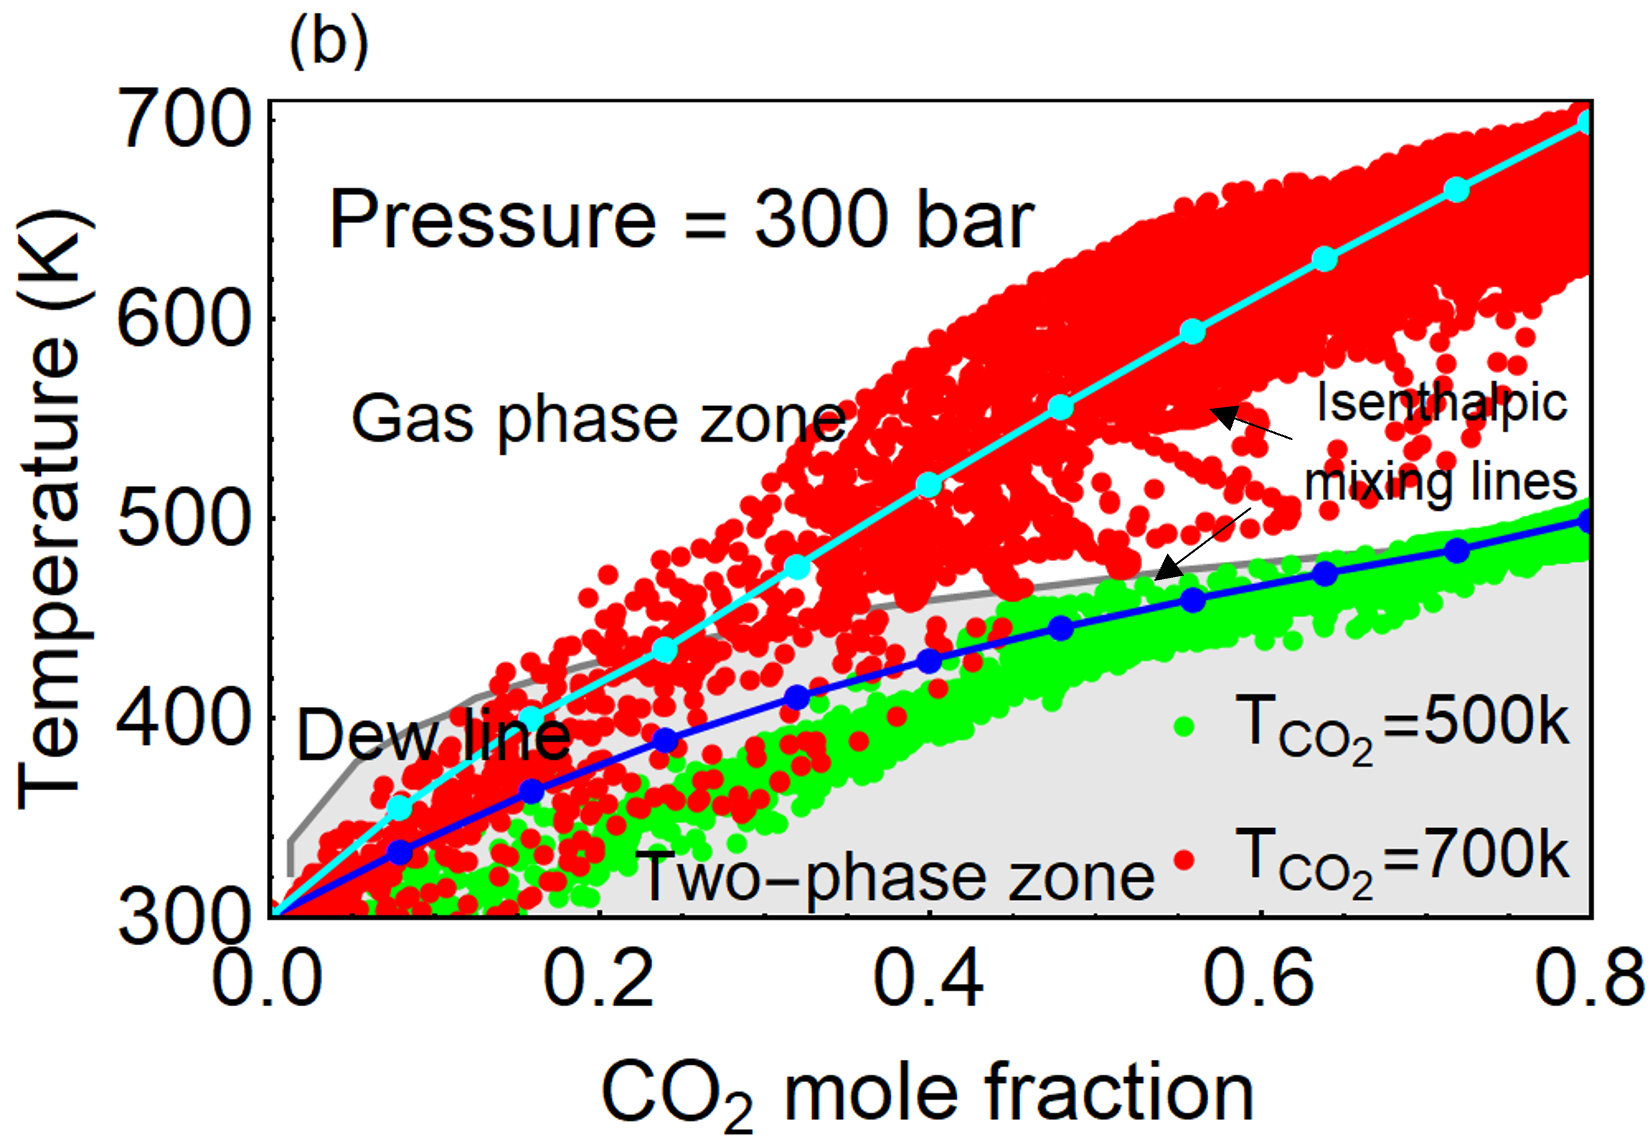
\includegraphics[width=0.45\linewidth]{Cof_n_u_v2_flow_c.png}
    }
    \caption{Temperature-component diagrams of the LES data of two jet-in-crossflows: (a) injecting \ce{CH4} into the \ce{CO2}/\ce{H2O} mixture with 20\% \ce{H2O}; (b) injecting \ce{O2} into the \ce{CO2}/\ce{H2O} mixture with 20\% \ce{H2O}.}
    \label{JICFT}
\end{figure}

\begin{figure}[htb]
    \centering
    \subfigure{
        \centering
        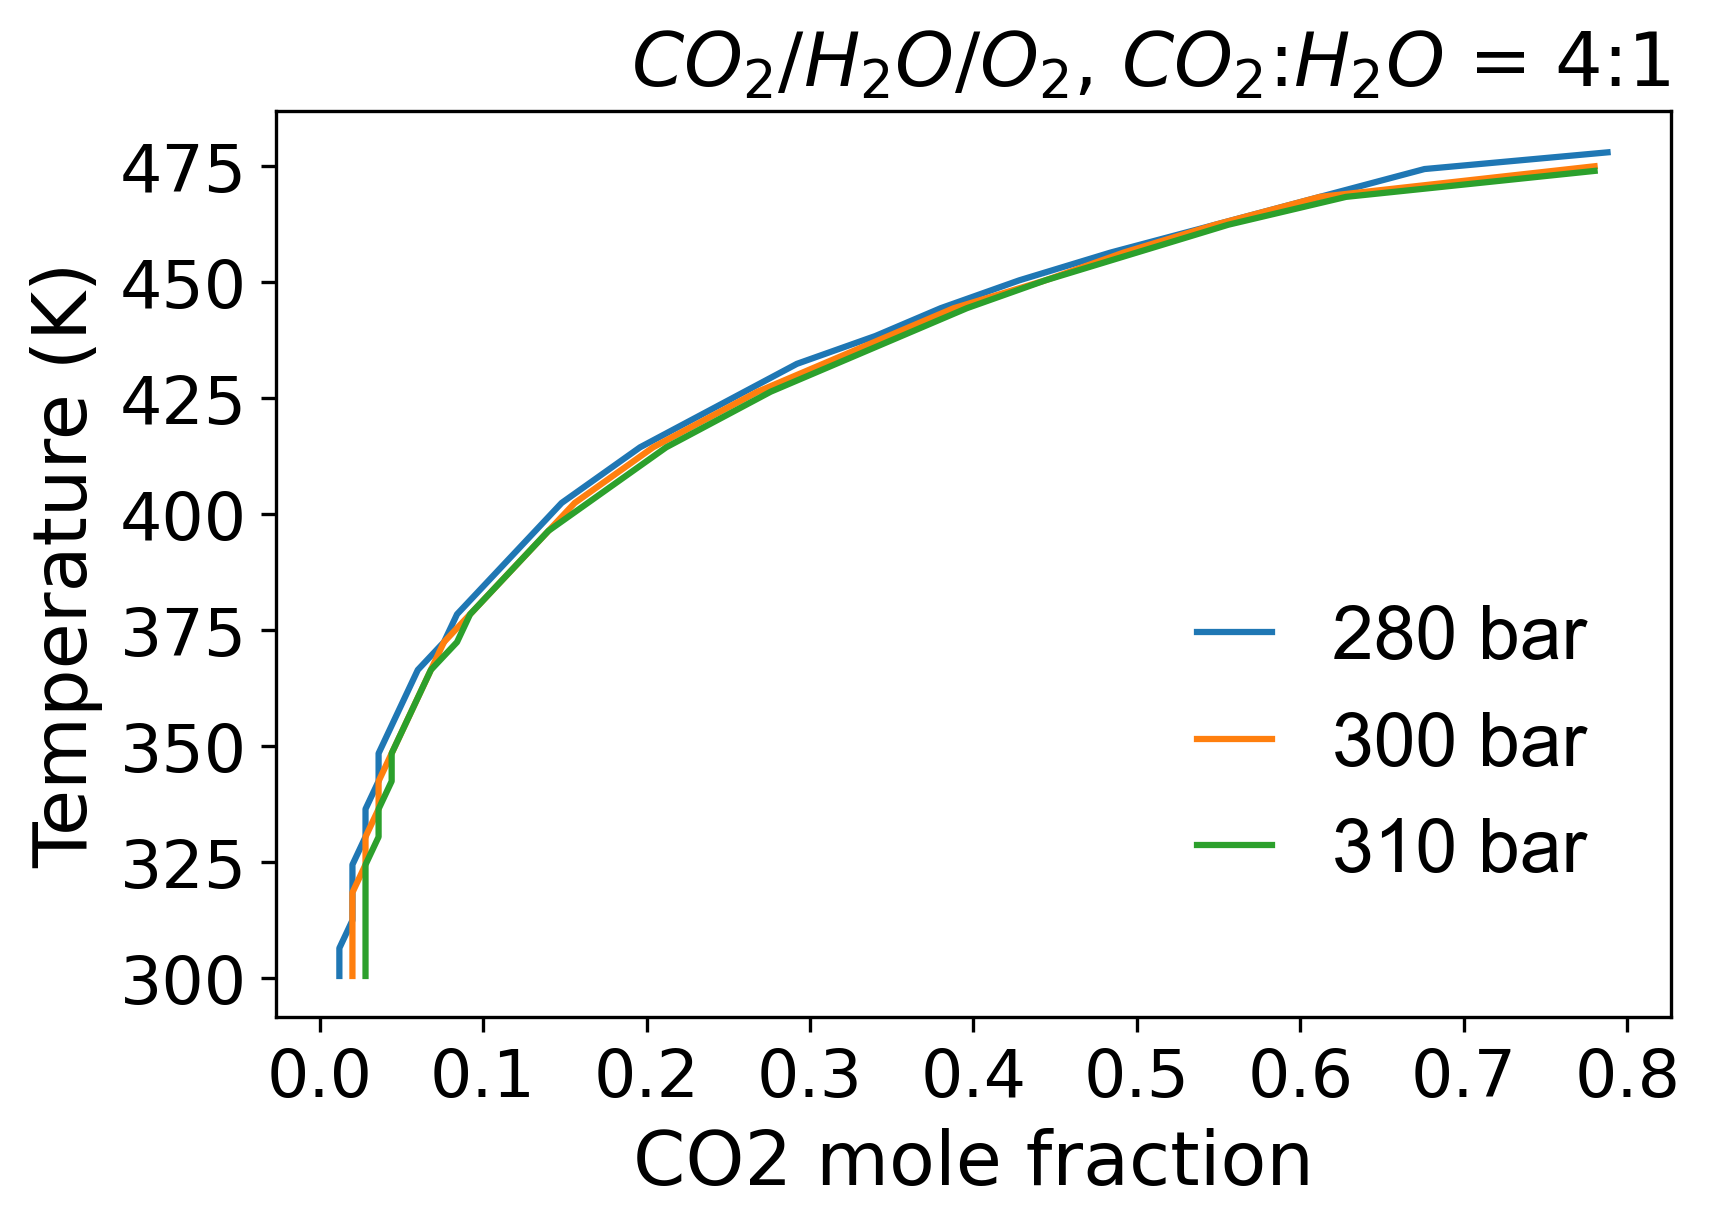
\includegraphics[width=0.45\linewidth]{TX.png}
    }
    \caption{Temperature-component diagrams of a \ce{CO2}/\ce{H2O}/\ce
    {O2} system at 280 bar, 300 bar, 310 bar. \ce{CO2}:\ce{H2O} = 4:1, by mole.}
    \label{JICFTX}
\end{figure}

Finally, the effect of \ce{H2O} addition is investigated. In this case, the ambient temperature is chosen as 500 K, and \ce{CO2} contains 10\% \ce{H2O} instead of 20\% in the previous LES cases. Comparing Fig.~\ref{JICFH}(a) with the previous result in Fig.~\ref{JICFr}(d), less \ce{H2O} leads to a smaller phase separation region. The mechanism behind this can be found in the phase diagram in Fig~\ref{JICFH}(b). The mixing trajectories almost overlap with the isenthalpic lines. The mixture \ce{CO2} with less \ce{H2O} has a lower dew line, and the high-temperature endpoint of the mixing trajectory moves out of the subcritical two-phase zone. The thermodynamic states of most fluid are near that endpoint. Hence, the subcritical two-phase zone in physical space is much smaller than the case with more \ce{H2O}.
\begin{figure}[htb]
    \centering
    \subfigure{
        \centering
        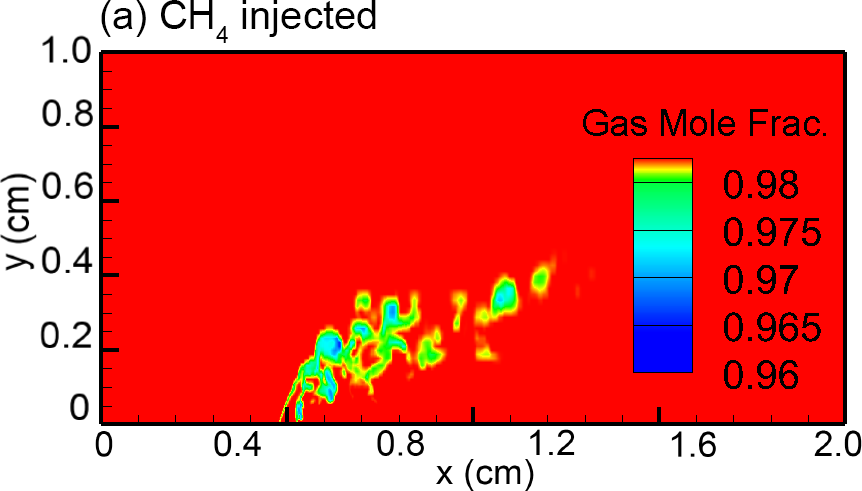
\includegraphics[width=0.5\linewidth]{3a_ps.png}
        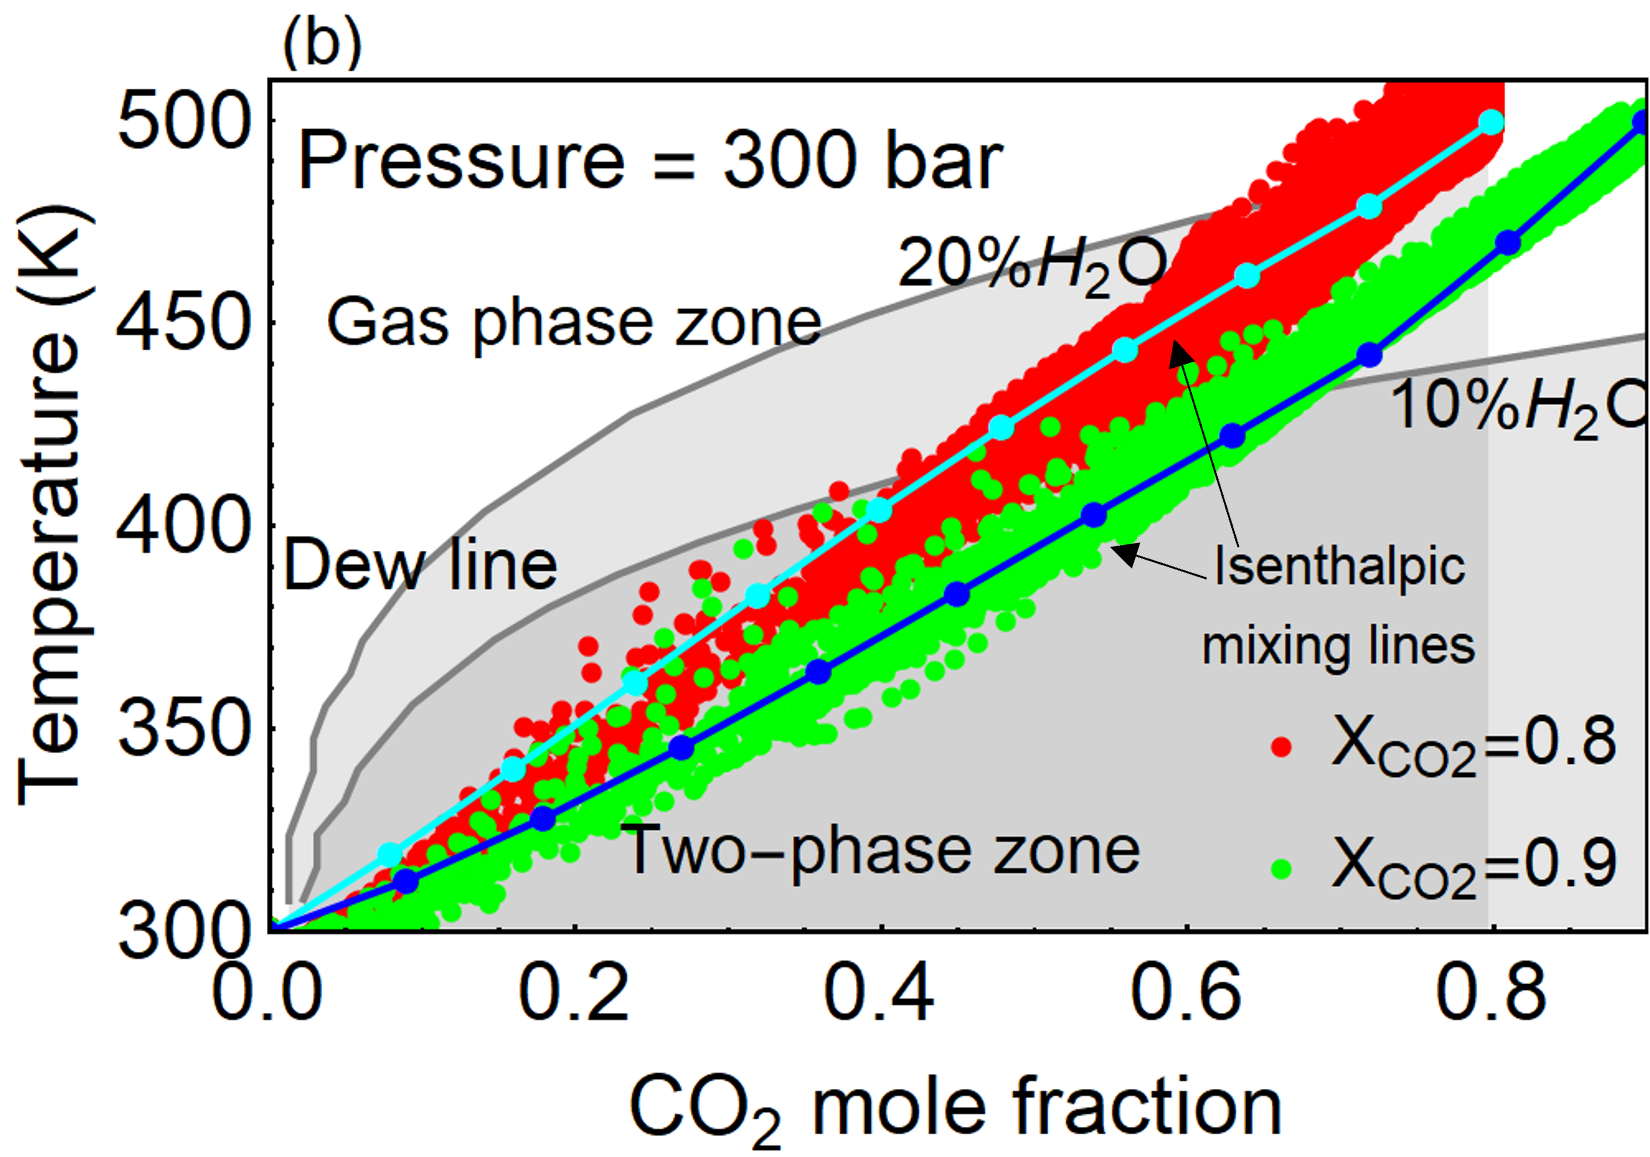
\includegraphics[width=0.4\linewidth]{Chf_n_u_v2_flow_c.png}
    }
    \caption{(a) LES of turbulent jet-in-crossflow of injecting \ce{CH4} into the \ce{CO2}/\ce{H2O} mixture with 10\% \ce{H2O} (ambient temperature is 700 K): (a) gas mole fraction, and (b) temperature-component phase diagram.}
    \label{JICFH}
\end{figure}

The conclusion is that when cold \ce{O2} or \ce{CH4} is injected into a hot mixture of \ce{CO2} and \ce{H2O}, phase separation may occur. This phenomenon requires the \ce{CO2}/\ce{H2O} mixture to be close to the subcritical two-phase zone. %, then distinct phase change can be observed. 
Hence, ambient temperature and \ce{H2O} concentration have an evident influence on the phenomenon. Thermodynamics analysis can only tell whether there is phase separation. In contrast, when the thermodynamics analysis is combined with the CFD simulation, more insights can be obtained about the location and mole fraction of the liquid phase formed during the mixing.



\section{Grid convergence test of jet-in-crossflow LES} \label{app:coverge}

    To test the grid convergence, two more meshes are created for comparison. Compared with the original mesh in Fig.~\ref{JICFg}, one mesh (denoted as the Mesh 1) contains half as many cells by evenly coarsening the original mesh in three directions (i.e., cells length scale $\sim \sqrt[3]{2}$ original cells length scale), and the other mesh (denoted as the Mesh 2) contains one-fourth of cells by evenly coarsening the original mesh (i.e., cells length scale $\sim \sqrt[3]{4}$ original cells length scale). The same jet-in-crossflow case as in Sec.~\ref{sec:results:combustor:HPn} (the \ce{CO2}/\ce{H2O} mixture is 700 K, and has 20\% \ce{H2O} by mole; \ce{O2} (300 K) is injected.) is simulated using the new meshes. After the results reach the statistically stationary state, the mean gas mole fraction and mean density averaged over 1 ms (physical time) are shown in Fig.~\ref{converge}. %All three meshes provide similar predictions in the qualitative sense, but the penetration length prediction contains small perturbation.
    To better quantify the difference between the three results, the relative differences based on $L^2$ norm are computed (relative difference of property $v$ is defined as $\left\|v-v_{orig}\right\|_{L^2}/\left\|v_{orig}\right\|_{L^2}$) and shown in Table~\ref{converge:error}. Since the results at the fields far from the injection nozzle are similar, the relative difference computation only uses the data near the nozzle (i.e., the dashed box in Fig.~\ref{converge} (in the top left sub-figure)). As seen, refining the grid by a factor of two almost does not change the relative difference, and the relative differences are stably maintained at $\sim$0.2\%, $\sim$5\% and $\sim$5\% for gas mole fraction, density, and temperature, respectively. Hence, in terms of the relative differences between grids shown in Table~\ref{converge:error}, the original grid resolution in this work is sufficient.
    

    \begin{figure}[htbp]
        \centering
        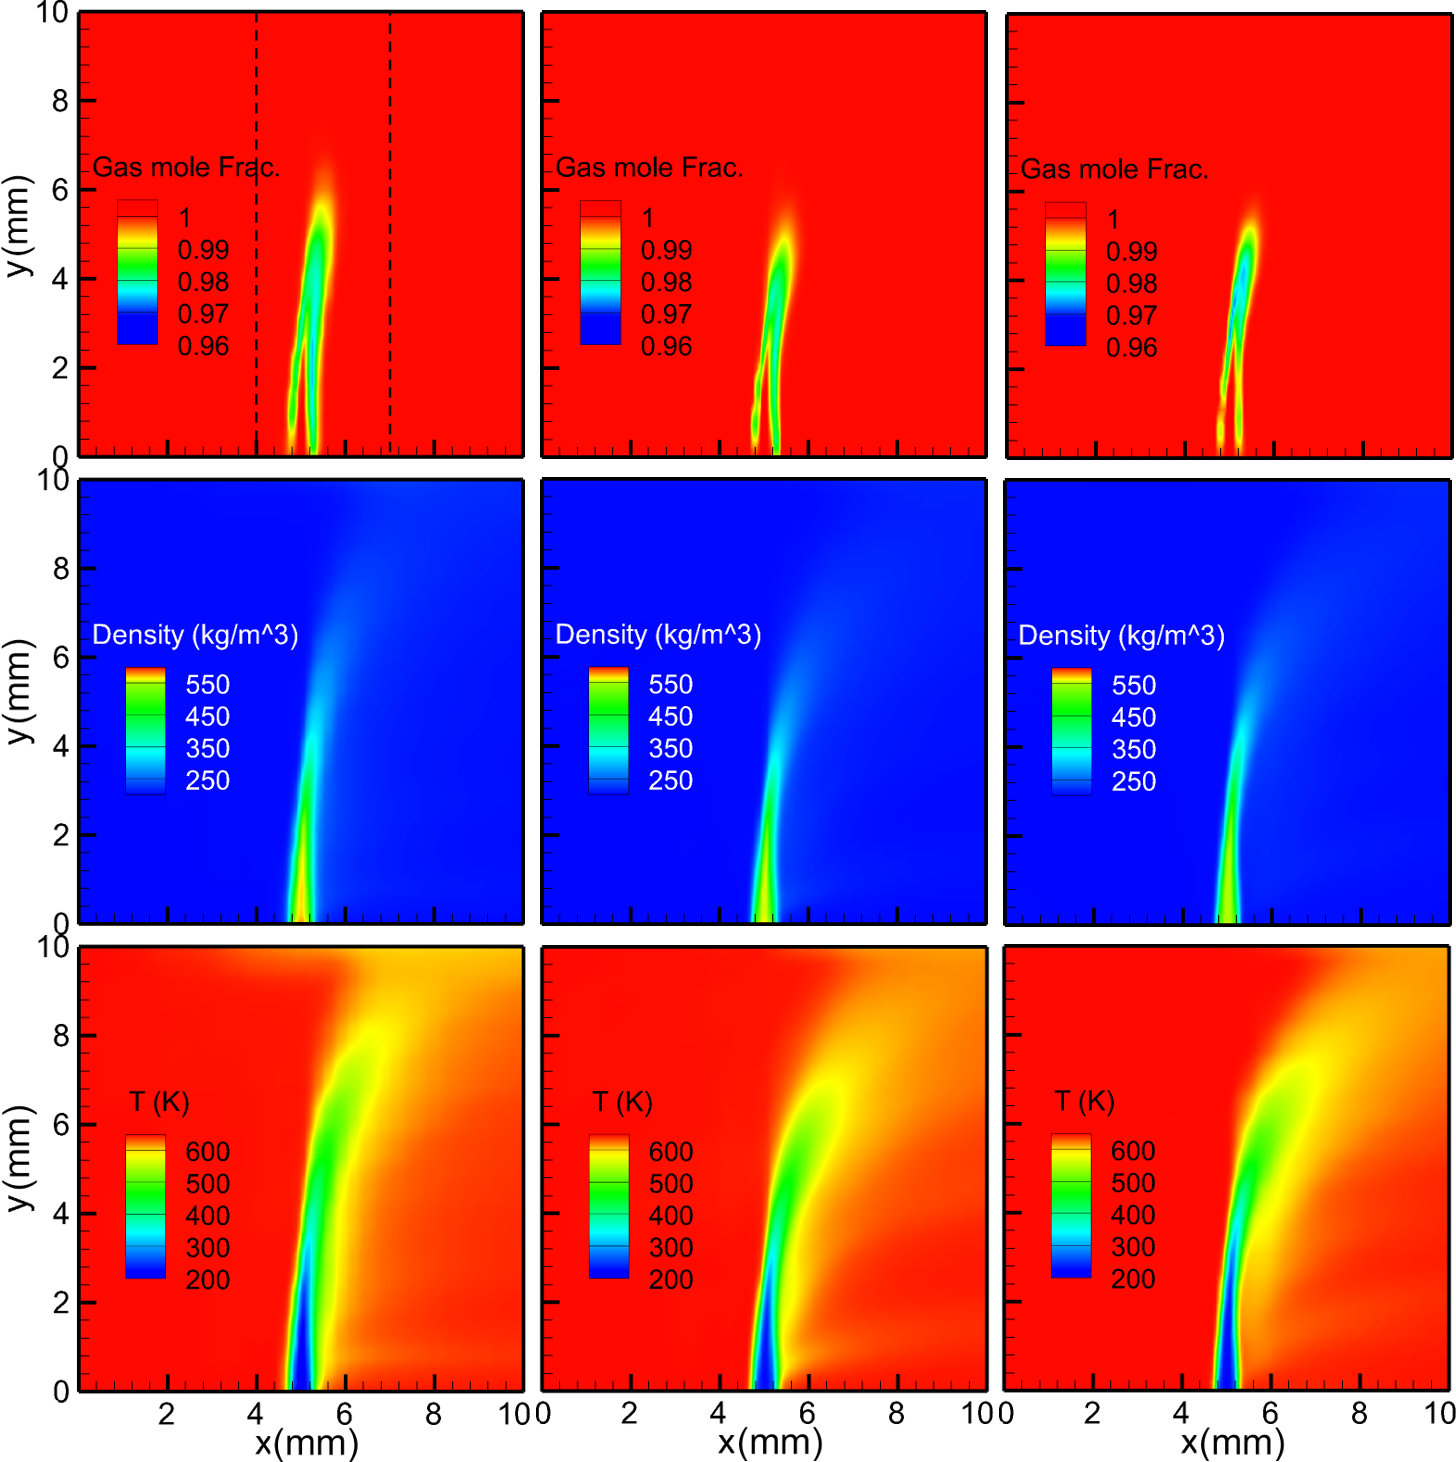
\includegraphics[width=1.0\linewidth]{9fig_c.png}
        \caption{Grid convergence test (the \ce{CO2}/\ce{H2O} mixture is 700 K, and has 20\% \ce{H2O} by mole, \ce{O2} (300 K) is injected.). Top: mean gas mole fraction, middle: mean density, bottom: mean temperature; left: Mesh 2, middle: Mesh 1, right: the original mesh.}
        \label{converge}
    \end{figure}

    \begin{table}[htbp]
        \centering
        \begin{minipage}{0.9\textwidth}
            \caption{Relative difference with respect to the original mesh (based on $L^2$ norm).} \label{converge:error}
            \begin{center}
                \begin{tabular}{@{}l|ll@{}} 
                    \toprule
                                      & Mesh 1   & Mesh 2   \\ 
                    \midrule
                    Gas mole fraction & 0.195\% & 0.256\% \\
                    Density           & 4.392\% & 7.149\% \\ 
                    Temperature       & 3.325\% & 5.737\% \\
                    \bottomrule
                \end{tabular}

            \end{center}
        \end{minipage}
        %\end{center}

    \end{table}

%%%%%%%%%%%%%%%%%%%%%%%%%%%%%%%%%%%%%%%%%%%%%%%%%%%%%%%%%%%%%%%%%%%%%%%%%%%%%%%%
